\documentclass[12pt]{article}
\usepackage[margin=1in]{geometry}
\usepackage{amsmath}
\usepackage{amssymb}
\usepackage{graphicx}
\usepackage{booktabs}
\usepackage[hidelinks]{hyperref}

\newcommand{\FDL}{\textnormal{[proved/checked finite-dimensional]}}
\newcommand{\CND}{\textnormal{[conditional]}}
\newcommand{\OBS}{\textnormal{[observed numerical evidence]}}
\newcommand{\OPN}{\textnormal{[open conjecture]}}
\newcommand{\CTX}{\textnormal{[counterexample]}}

\title{Pose-Confounding Spectral Geometry for Full-Wave Inverse-Scattering SLAM:
A Finite-Dimensional Numerical Study}
\author{Inv-SLAM idea-loop experiment synthesis (executable-record draft)}
\date{2026-09-03}

\begin{document}

\maketitle

\begin{abstract}
We study local observability of a volumetric material-contrast map when the
transmitting and receiving platform pose is unknown, using only the
finite-dimensional checks that were actually executed in this working
directory. Starting from a two-dimensional scalar Helmholtz contrast-source
model, we build whitened and realified map and pose Jacobians $A$ and $B$, and
compare the known-pose information $K_{\mathrm{IS}}=A^TA$ with the
pose-eliminated information
$K_{\mathrm{SLAM}}=A^T P_{\mathrm{Range}(B)^\perp}A$ and its finite-prior
Schur complement $K_{\mathrm{eff}}$. The checked finite-dimensional theory
links exact map--pose ambiguity to $\mathrm{Range}(A)\cap\mathrm{Range}(B)$,
identifies the no-prior generalized retention spectrum with squared sines of
principal angles, and bounds information loss by the pose dimension. We report
the numerical consequences from five experiment families and their parent
corrections: analytic-Jacobian checks and grid diagnostics; kernel, rank,
retention, prior, and duplicate-block algebra; gauge and Born-empty-background
controls; frequency and equal-budget trajectory comparisons; and first-order
sensitivity tests with rank-event caveats. An additional round of six
families and controls extends this record with a declared per-frequency
colored-noise whitening model; a same-standoff, per-pose-energy-normalized
trajectory control; resolution and rank-event diagnostics on finite grids; an
explicit current-space versus map-tangent composition check; and a derived
alpha-aware operator-Lipschitz bound for the affine tangent model. The same
scope discipline applies to these additions: the whitening, algebraic,
containment, and affine-certificate statements are finite-dimensional checks;
the mode, trajectory, and sweep distinctions are recorded observations; and
the surviving counterexamples and boundary events are preserved rather than
forced to pass. The study retains its recorded
counterexamples: these numerical results validate the algebraic implementation
and refine or falsify proposed physical generalizations on the tested discrete
scenario, but they cannot establish continuum transfer, global nonlinear
convergence, online SLAM performance, or global novelty.
\end{abstract}

\tableofcontents

\section{Introduction and contributions}\label{sec:intro}

Simultaneous localization and mapping (SLAM) from coherent full-wave
measurements couples a map of material contrast to the unknown poses at which
the scene is probed. When the underlying forward model is a nonlinear inverse
scattering map, the standard information-theoretic reduction first linearizes
about a nominal contrast and trajectory, whitens the measurement noise, and
realifies the parameters so that real pose increments act on real degrees of
freedom. Eliminating the pose nuisance then produces an effective
map-information operator whose local geometry can be characterized by
finite-dimensional linear algebra.

The contribution of this draft is deliberately bounded:
\begin{itemize}
\item We formulate and test an explicit finite-dimensional theory in which
the pose-induced information loss is low rank, the no-prior normalized
retention spectrum equals the squared-sine principal-angle spectrum between
the map and pose data tangents, and finite-prior retention is a weighted
Schur-complement shrinkage. These statements are elementary and are labelled
\FDL{}; they are verified on the discrete harness recorded here, not on the
continuum problem.
\item We execute the round-1 and round-2 experiment families and controls on
one Apple Silicon CPU harness with deterministic seeds, machine-precision rank
tolerances, exact commands, hashes, and raw JSON records, and we keep the
failures and counterexamples exactly as recorded (Sections~\ref{sec:results}
and Appendix~\ref{app:claims}). The round-2 results appear in
Sections~\ref{sec:family6}--\ref{sec:family5b2}.
\item We state the boundary explicitly: no continuum transfer, global
nonlinear convergence, online SLAM performance, or global novelty is claimed
(Section~\ref{sec:limits}). Retrieval-bounded related work is discussed in
Section~\ref{sec:related}; this draft never asserts ``first'' or ``no prior
work.''
\end{itemize}

All matrix identities below are stated in the whitened/realified data space
with real map and pose parameters. The results are local and information-
theoretic; they concern local observability and Fisher-type information, not
estimation, recovery, or decision performance.

\section{Model, whitening/realification, and information operators}\label{sec:model}

\subsection{Discrete contrast-source model}

The scenario is a deterministic, synthetic two-dimensional scalar Helmholtz
contrast-source problem on $D=[-0.5,0.5]^2$ discretized on a uniform $N\times
N$ grid with step $h=1/N$. Let $k_b$ be the background wavenumber and
$\chi$ the relative contrast
\[
\chi(r)=\frac{k^2(r)-k_b^2}{k_b^2},
\]
so that the contrast is dimensionless. The free-space Green function is
\[
g_k(r,r')=\frac{i}{4}H_0^{(1)}(k_b|r-r'|),
\]
with gradient convention
\[
\nabla_r g_k(r,r')=-\frac{i k_b}{4}H_1^{(1)}(k_b R)\frac{r-r'}{R},\qquad
R=|r-r'|.
\]
For the equal-area disk cell of radius $a=h/\sqrt{\pi}$, the domain-propagator
diagonal uses the complete disk integral \FDL{} (corrected 2026-09-03, see
Section~\ref{sec:family1}):
\[
I_{\mathrm{self}}=\frac{i\pi a}{2k_b}H_1^{(1)}(k_b a)-\frac{1}{k_b^2},\qquad
[G_D]_{nn}=k_b^2 I_{\mathrm{self}}.
\]
The linearized state operator is $M_t=I-D_\chi G_{D,t}$ with the total field
defined through the contrast-source Lippmann--Schwinger equation, and the
current-eliminated forward map is $F(\chi,X)=G_S M^{-1} D_\chi E^{\mathrm{inc}}$
for a trajectory $X=(x_1,\ldots,x_T)$ of poses $x_t=(p_x,p_y,\theta)\in
\mathrm{SE}(2)$.

\subsection{Whitening and realification}

For a covariance model with whitening factor $W$, the complex-valued Jacobians
are converted to real matrices of doubled row count,
\[
A_R=\sqrt{2}\begin{bmatrix}\Re(WA)\\\Im(WA)\end{bmatrix},\qquad
B_R=\sqrt{2}\begin{bmatrix}\Re(WB)\\\Im(WB)\end{bmatrix},
\]
where $A=D_\chi F$ is the map Jacobian and $B=D_X F$ is the pose Jacobian.
All projectors, ranks, principal angles, Schur complements, and spectra in
this draft are computed after this conversion. Complex-linear projectors
$BB^+$ acting on real pose increments would enlarge the nuisance range and
overestimate map--pose confounding; they are not used. In the executed runs
$W$ is the identity ($W=I$) except where a declared block-normalization or
SNR-matched control rescales rows per frequency block.

\subsection{Information operators}

In the whitened/realified space, with $m$ real data rows and $q$ real pose
columns, define the known-pose map information, the no-prior pose-eliminated
information, and the finite-prior Schur complement by
\begin{align}
K_{\mathrm{IS}}&=A^T A,\\
K_{\mathrm{SLAM}}&=A^T P_{\mathrm{Range}(B)^\perp}A
=A^T(I-BB^+)A,\\
K_{\mathrm{eff}}(\alpha)&=A^TA-A^TB\,(B^TB+\alpha I)^{-1}B^TA,
\qquad \alpha\ge 0,
\end{align}
where the $q\times q$ system is solved stably. The pose-induced loss is
$L_X=K_{\mathrm{IS}}-K_{\mathrm{eff}}$. For no prior the generalized retention
spectrum is obtained from $Q_A^T P_{\mathrm{Range}(B)^\perp}Q_A$ with
orthonormal bases $Q_A$ and $Q_B$ of $\mathrm{Range}(A)$ and
$\mathrm{Range}(B)$: with descending singular values of $Q_B^TQ_A$, the
retentions are reported in ascending order as
\[
\rho_i=1-\sigma_i^2(Q_B^TQ_A),
\]
padded with $\rho_i=1$ in unmatched directions. This is the
\FDL{} identity $K_{\mathrm{SLAM}}v=\rho K_{\mathrm{IS}}v$ on the observable
support of $K_{\mathrm{IS}}$ expressed through principal angles.

The executed algebraic statements, all \FDL{}, are:
\begin{enumerate}
\item $\ker K_{\mathrm{SLAM}}=\{u: Au\in \mathrm{Range}(B)\}$ (including
$\ker A$).
\item $\mathrm{rank}\,K_{\mathrm{IS}}-\mathrm{rank}\,K_{\mathrm{SLAM}}=
\dim(\mathrm{Range}(A)\cap\mathrm{Range}(B))$.
\item $0\le K_{\mathrm{SLAM}}\le K_{\mathrm{IS}}$, and at most
$\mathrm{rank}(B)$ generalized retention values differ from $1$.
\item $\mathrm{rank}\,L_X\le \mathrm{rank}(B)$, with Hermitian interlacing
between $K_{\mathrm{IS}}$, $K_{\mathrm{eff}}(\alpha)$, and $K_{\mathrm{SLAM}}$.
\item Along a fixed-rank regular path $J_X=\alpha I$, $K_{\mathrm{eff}}\to
K_{\mathrm{SLAM}}$ as $\alpha\to0$ and $K_{\mathrm{eff}}\to K_{\mathrm{IS}}$
as $\alpha\to\infty$, on the tested support. A singular-support prior (an
unpenalized pose direction) prevents convergence to $K_{\mathrm{IS}}$
(\CND{} + \FDL{} on the recorded finite geometry).
\item Duplicating data as $A_{\mathrm{aug}}=[A;cA]$,
$B_{\mathrm{aug}}=[B;cB]$ scales $K_{\mathrm{IS}}$ and $K_{\mathrm{SLAM}}$ by
$1+c^2$ and leaves the no-prior retentions unchanged; with a fixed finite
prior the data-to-prior weighting changes and retentions generally move; a
jointly scaled prior $J_X^{\mathrm{aug}}=(1+c^2)J_X$ restores invariance.
\end{enumerate}

For a full-wave model at zero background $\chi_0=0$, the first-order pose
Jacobian vanishes ($B=0$) so $K_{\mathrm{SLAM}}=K_{\mathrm{IS}}$; pose effects
then first appear through the bilinear term $(D_X A[\delta X])\delta\chi$,
which the runs evaluate rather than declare harmless.

\section{Experiment design}\label{sec:design}

\subsection{Unified harness and scenario}

One deterministic harness in \texttt{src/} implements the forward model, the analytic
Jacobian builders, whitening/realification, and the algebraic checks. The
nominal scene is the two-Gaussian contrast
$\chi_0=0.3\,\chi_{\mathrm{disk},1}+0.5\,\chi_{\mathrm{disk},2}$ used by
Family~1 with centers $(-0.15,-0.12)$ and $(0.18,0.14)$, widths
$\sigma=(0.09,0.07)$; $k_b=2\pi$; $T=6$ poses; and $n_{\mathrm{rx}}=4$
body-fixed receivers per pose, giving $m=48$ real data rows and $q=18$ pose
columns after realification. The pilot grid is $N=16$; N=24/32/40 runs are
recorded as refinement diagnostics. Two map parameterizations are analyzed:
the $N^2$-column pixel basis and a $p=24$ smooth Gaussian-RBF basis with unit
columns (4$\times$6 lattice, $\sigma_b=0.16$).

\subsection{Five families and parent corrections}

\begin{enumerate}
\item Family 1 verifies the corrected self-cell rule, direct radial
quadrature, source-gradient sign, centered map/pose finite differences, state
margin, Born/full-wave continuation, and a forward-model grid-refinement
diagnostic.
\item Family 2 checks the kernel/rank/retention identities, loss rank and
interlacing, prior sweeps, singular-prior limits, duplicate-block rules, and
smooth-basis resolution persistence. Parent corrections added a stable
$C^TC$ factorization check and an SVD-filtered small-prior sweep.
\item Family 3 tests smooth-basis and pixel-basis SE(2) gauge cancellation,
kernel distances, anchor/symmetry controls, and Born-empty-background
degeneration. Family 3b reruns the same claims under corrected validity
conditions (generator-representing augmented basis, generator-specific
retention, and genuinely small scene amplitudes) without modifying the raw
Family 3 record.
\item Family 4 stacks genuinely distinct frequency blocks with one shared
pose compensation, checks PSD monotonicity and duplicate controls, and
compares four equal-budget trajectories. Family 4b adds a declared
block-normalized control; the parent controls add an SNR-matched frequency
control and equal-length/same-radius trajectory orderings.
\item Family 5 verifies full trajectory/eigenvalue derivative formulas against
finite differences, quantifies the frozen-nuisance error, tests a robust
first-order surrogate, records an empirical-only Weyl/Lipschitz self-check,
and scans a random path for near-crossings and rank events.
\end{enumerate}

\paragraph{Round-2 families and their roles.}
\begin{itemize}
\item Family 6 declares a per-frequency colored-noise covariance with a
receiver Mat\'ern-1/2 factor and per-frequency SNR-matched whitening, and
reruns whitening sanity, algebraic-spine, duplicate-block, and stacking
checks under the declared colored-whitened blocks (colored-noise control).
\item Family 4c holds curved-path standoff fixed and equalizes each pose's
realified $A$-block energy before projection, so trajectory geometry is
compared after removing radius/standoff and per-pose signal-strength scaling
(trajectory and standoff control).
\item Family 7 records resolution, frequency-rank, near-crossing, and
Born-to-full-wave contrast diagnostics on finite grids (continuum/rank
diagnostics only, not a continuum proof).
\item Family 8 makes the current-space $G_S$/SOM and map-tangent
$A$/$K_{\mathrm{eff}}$ objects explicit in the same pixel space and checks
their composition identity, range containment, and mode-subspace distinction
(SOM/current-space distinction).
\item Family 9 reruns the algebraic-spine and frequency-diversity claims over
seven scenes and records pose-DOF, receiver-count, pose-count, and
smooth-basis ablations (replications and component ablations).
\item Family 5b2 derives an alpha-aware structural operator-Lipschitz bound
for the affine tangent model and verifies the certificate on 2000 directions;
the loose Family 5b precursor is cited only as corrected by Family 5b2
(Lipschitz certification).
\end{itemize}

\subsection{Tolerances, seeds, and environment}

Rank tolerance for exact algebraic checks is
$\tau(M)=\max(m,n)\,\epsilon_{\mathrm{machine}}\,\sigma_1(M)$. PSD and
interlacing violations are rejected above
$-10^{-10}\max(1,\|K_{\mathrm{IS}}\|_2)$; the c1 subspace gate is
$10^{-8}\max(1,\|A\|_2^2)$; c3 prediction residual gate is
$10^{-10}\max(1,\|A\|_2^2)$; c8 invariance gates are $10^{-10}$. Deterministic
seeds are recorded per run (map seeds $\{0,1,2\}$, pose seeds
$\{10,11,12\}$, gauge Born seed 31415, Family 5 perturbation seeds
2718/9191/150 samples, etc.). All runs execute on Apple Silicon CPU only
(macOS-26.6.2 arm64), Python 3.12.13, numpy 2.5.2, scipy 1.18.1, matplotlib
3.11.1; no GPU/MPS/CUDA, no network services, and no random draws except the
declared fixed seeds.

\section{Results}\label{sec:results}

Each subsection reports the key numbers from the recorded JSONs followed by
the preserved negative results and counterexamples. Statuses are quoted
exactly as executed; Appendix~\ref{app:claims} repeats the claim-status
tables. Figure files produced by the runs are listed in the reproducibility
section.

\subsection{Family 1: forward model and corrected analytic Jacobians}\label{sec:family1}

The initial Family-1 implementation used an invented self-cell rule that
omitted the lower endpoint of the Hankel antiderivative
($\lim_{x\to0}xH_1^{(1)}(x)=-2i/\pi$), so the alleged disk integral tended to
$1/k_b^2$ instead of zero as $h\to0$. The pre-correction snapshot is preserved
verbatim under \texttt{archive/INVALIDATED\_self\_cell\_2026-09-03T092339Z/}. The
corrected rule
$I_{\mathrm{self}}=i\pi a H_1^{(1)}(k_ba)/(2k_b)-1/k_b^2$ matches 2048-node
radial quadrature to max absolute error $3.13\times10^{-16}$, with
$|I_{\mathrm{self}}|$ dropping monotonically from $5.12\times10^{-3}$
(N=8) to $4.36\times10^{-5}$ (N=128); the invalidated rule stays near
$2.5\times10^{-2}$. The source-gradient identity
$\nabla_s g=-\nabla_z g$ is unit-tested against finite differences in the
source coordinate (corrected relative error $1.7\times10^{-9}$ versus
$2.0$ for the old sign).

\begin{table}[ht]
\centering
\small
\caption{Family 1 key numbers (recorded in
\texttt{results/family1\_pilot\_results.json} and
\texttt{results/family1\_grid\_refinement.json}).}
\label{tab:f1}
\begin{tabular}{l l}
\toprule
quantity & value \\
\midrule
map-FD rel.\ error at h=$10^{-3}$ (seeds 0/1/2) &
$2.25\times10^{-9}$ / $1.74\times10^{-8}$ / $1.77\times10^{-9}$ \\
pose-FD rel.\ error at h=$10^{-3}$ (seeds 10/11/12) &
$8.38\times10^{-7}$ / $4.28\times10^{-6}$ / $4.09\times10^{-6}$ \\
map slope / pose slope (5-pt window) &
1.976 (r$^2$=0.9998) / 2.0000 (r$^2$=1.0000) \\
state margin $\sigma_{\min}(M)/\|M\|_2$; max residual &
0.7189; $9.34\times10^{-16}$ \\
Born/full-wave rel.\ discrepancy, s=0.01..0.2 &
F: $1.77\times10^{-3}$..$3.54\times10^{-2}$; A-Fro: $1.89\times10^{-3}$..$3.82\times10^{-2}$ \\
grid rel.\ difference vs N=40 (N=16/24/32) &
$1.453\times10^{-3}$ / $5.030\times10^{-4}$ / $1.601\times10^{-4}$ \\
\bottomrule
\end{tabular}
\end{table}

The Family-1 checks are \FDL{} internal consistency and quadrature-fidelity
checks of the implemented discrete solver. The grid refinement is a forward-
model diagnostic: the successive differences shrink monotonically, but the
grids are not a nested restriction of one continuum problem, so no continuum
convergence is claimed.

\subsection{Family 2: algebraic spine}\label{sec:family2}

Family 2 verifies the Section~\ref{sec:model} identities on the discrete
(whitened/realified) Jacobian pair in both the pixel basis
($n=256$, $\mathrm{rank}(A)=48=m$) and the smooth basis ($n=p=24$,
$\mathrm{rank}(A)=24$); both share $\mathrm{rank}(B)=18$.

\begin{table}[ht]
\centering
\small
\caption{Family 2 key numbers (pixel / smooth; \texttt{results/family2\_results.json}
and \texttt{results/family2\_parent\_correction.json}).}
\label{tab:f2}
\begin{tabular}{l l}
\toprule
quantity & value \\
\midrule
c1 pixel projector subspace distance vs $10^{-8}$ gate &
$8.47\times10^{-7}$; \texttt{pass\_gate=false}, \texttt{identity\_support=true} \\
c1 smooth subspace distance & 0 \\
identity-support evidence (pixel) &
nullity 226=226; $\sigma_{\min}(N_1^TN_2)=1-4\times10^{-13}$; \\
 & $\max\|K_{\mathrm{SLAM}}N_2\|=1.96\times10^{-19}$ \\
c2 rank residuals & 0 (pixel and smooth) \\
c3 retention residual $\max|\rho-\rho_{\mathrm{pred}}|$ &
$2.89\times10^{-15}$ / $1.55\times10^{-15}$ \\
count $\rho<1$ & 18 = 18 = $r_B$ (both bases) \\
c4 stable-factor rank $L_X$ & 18 = $r_B$ (both) \\
c5 PSD minima / interlacing violations &
$\ge -2.5\times10^{-19}$ / $-2.9\times10^{-20}$; \\
 & max positive violation $5.0\times10^{-21}$ / $6.7\times10^{-21}$ \\
c6 d0 at $\alpha=10^{-6}$ (grid left edge) & 0.209 / 0.137 \\
c6 SVD-filter d0 at $\alpha=10^{-14}$ (parent correction) &
$5.70\times10^{-9}$ / $3.67\times10^{-9}$ \\
c6 dinf at $\alpha=10^{4}$ & $5.17\times10^{-7}$ / $5.50\times10^{-7}$ \\
c7 singular-prior dinf at $\alpha=10^{4}$ &
$4.71\times10^{-4}$ / $2.30\times10^{-4}$ (417-912x regular) \\
stable kernel-factorization residual &
$3.77\times10^{-16}$ / $2.70\times10^{-16}$ \\
duplicate fixed-prior rho change ($\alpha=1$) &
$3.99\times10^{-2}$ / $3.98\times10^{-2}$ \\
\bottomrule
\end{tabular}
\end{table}

\paragraph{Preserved negative result (c1 pixel).}
The pixel-basis null space of $K_{\mathrm{SLAM}}$ is 226-dimensional, and any
eigh-based orthonormal basis of the zero cluster mixes at the
$\sim\epsilon\|K_{\mathrm{SLAM}}\|/\mathrm{gap}$ level because the smallest
positive singular value of $K_{\mathrm{SLAM}}$ is $\sim1.2\times10^{-14}$. The
subspace distance $8.47\times10^{-7}$ therefore exceeds the predeclared
$10^{-8}$ projector gate; the gate is recorded as failed. The identity
$\ker K_{\mathrm{SLAM}}=\{u:Au\in\mathrm{Range}(B)\}$ is nevertheless certified
by equal nullities (226=226), by the residuals
$\max\|K_{\mathrm{SLAM}}N_2\|=1.96\times10^{-19}$ and
$\max\|C N_1\|=1.56\times10^{-13}$, by
$\sigma_{\min}(N_1^TN_2)=1-4\times10^{-13}$, and by the stable factorization
$K_{\mathrm{SLAM}}=C^TC$ with relative residual $3.77\times10^{-16}$.

\paragraph{Preserved caveats (c6/c7).}
On the planned grid, $\alpha=10^{-6}$ is not asymptotic for this geometry
because $\sigma_{\min}(B_R)^2\approx4.6\times10^{-7}<\alpha$; the recorded
statement is the monotone limiting behaviour, confirmed to
$d_0=5.70\times10^{-9}$/ $3.67\times10^{-9}$ at $\alpha=10^{-14}$ by the
SVD-filtered parent-correction sweep. The singular-prior direction (pose
column 18, last pose theta) is an unpenalized nuisance coordinate, explicitly
not called a gauge; its nonzero limiting relative loss is
$4.71\times10^{-4}$/ $2.29\times10^{-4}$, below the illustrative $0.1$ level
because that direction has modest data sensitivity in this geometry.

\subsection{Family 3: gauge and Born empty-background degeneration}\label{sec:family3}

The raw record (\texttt{results/family3\_gauge\_born.json}) preserves the following
results exactly.

\begin{table}[ht]
\centering
\small
\caption{Family 3 raw key numbers
(\texttt{results/family3\_gauge\_born.json}). Pixel residuals are N=16.}
\label{tab:f3}
\begin{tabular}{l l l}
\toprule
quantity & smooth basis & pixel basis \\
\midrule
gauge residual Tx & $1.83\times10^{-1}$ & $6.61\times10^{-5}$ \\
gauge residual Ty & $8.65\times10^{-2}$ & $1.58\times10^{-5}$ \\
gauge residual Rot & $3.10\times10^{-1}$ & $4.68\times10^{-5}$ \\
representation residual (Tx/Ty/Rot) &
0.781 / 0.572 / 0.703 & 0 \\
kernel distance (Tx/Ty/Rot) &
$1.91\times10^{-8}$/$2.31\times10^{-9}$/$1.43\times10^{-8}$ &
$3.96\times10^{-10}$/$8.73\times10^{-11}$/$1.85\times10^{-10}$ \\
anchor $\rho_{\min}$ ratios (corner/disk/boundary) &
1.26 / 0.011 / 0.244 & --- \\
Born empty background $\|B_0\|_F$ and
$\|K_{\mathrm{SLAM},0}-K_{\mathrm{IS},0}\|_F/\|K_{\mathrm{IS},0}\|_F$ &
0.0 and 0.0 & --- \\
raw full-wave rel.\ error at h=$10^{-3}$ (O(1) unit-L2 scene) &
0.218 (h-independent) & --- \\
\bottomrule
\end{tabular}
\end{table}

\paragraph{Preserved failures.} The smooth-basis gauge gate
(residual $\le5\times10^{-2}$, decreasing to N=40) failed: Tx residual stayed
at $0.183\to0.183$, Ty at $0.0865$, Rot at $0.310\to0.309$, because the
analytic generator fields are not in the span of the p=24 RBF family
(representation residuals 0.78/0.57/0.70). The kernel-distance check is
therefore nonzero at $10^{-8}$-$10^{-9}$, not a gauge-level roundoff. The
global-$\rho_{\min}$ anchor prediction also failed for the three specified
masks (corner ratio only 1.26; disk and boundary ratios 0.011 and 0.244,
i.e., decreases). At Born empty background the algebra holds ($B=0$ and
$K_{\mathrm{SLAM},0}=K_{\mathrm{IS},0}$ to relative Frobenius 0.0), and the
bilinear term dominates the linear Born term by factor 2.81 at h=$10^{-3}$;
however, the specified full-wave finite-difference comparison at a unit-L2
scene has an h-independent mismatch floor of $2.18\times10^{-1}$ from
$\chi^2$-order pose derivatives, with remainder slope 1.015 rather than two.
These raw failures are not relabelled.

\subsection{Family 3b: corrected-condition refinement}\label{sec:family3b}

Family 3b (supplementary, \texttt{results/family3b\_refinements.json}) does not
supersede the raw Family 3 record. Its corrected conditions were: (A) pixel
discrete tangent; (B) p=27 smooth basis augmented with the generator fields;
(C) generator-specific retention instead of global $\rho_{\min}$; (D)
genuinely small scene amplitude $\|\delta\chi\|_2=10^{-3}$.

\begin{table}[ht]
\centering
\small
\caption{Family 3b key numbers (\texttt{results/family3b\_refinements.json}).}
\label{tab:f3b}
\begin{tabular}{l l}
\toprule
quantity & value \\
\midrule
pixel gauge residuals Tx/Ty/Rot at N=16/32/40 &
Tx $6.61\times10^{-5}$/$7.95\times10^{-5}$/$8.14\times10^{-5}$; \\
 & Ty $1.58\times10^{-5}$/$2.11\times10^{-5}$/$2.17\times10^{-5}$; \\
 & Rot $4.68\times10^{-5}$/$6.07\times10^{-5}$/$6.24\times10^{-5}$ \\
pixel kernel distances Tx (N16/32/40) &
$3.96\times10^{-10}$/$1.22\times10^{-10}$/$8.05\times10^{-11}$ \\
augmented p27 representation residual (Tx/Ty/Rot) &
$1.42\times10^{-15}$/$2.04\times10^{-15}$/$1.63\times10^{-15}$ \\
augmented p27 gauge residual (Tx/Ty/Rot) &
$6.61\times10^{-5}$/$1.58\times10^{-5}$/$4.68\times10^{-5}$ \\
base / corner-anchor generator $\rho_g$ &
$9.908\times10^{-11}$ / $1.182\times10^{-9}$ (ratio 11.93) \\
known-disk / outer-ring $\rho_g$ (reported, not forced) &
$2.165\times10^{-5}$ (ratio $2.19\times10^5$) / \\
 & $1.645\times10^{-8}$ (ratio 166) \\
$A(0)$ vs Born relative Frobenius &
$7.05\times10^{-17}$ global; $7.09\times10^{-17}$ max per pose \\
Born rel.\ error at h=$10^{-3}$ &
$2.27\times10^{-13}$ (value gate passes) \\
full-wave chi$^2$ floor & $2.166\times10^{-4}$ at every h (slope 5.4e-5) \\
remainder drift slope & 1.986 (r$^2=0.99999$) \\
\bottomrule
\end{tabular}
\end{table}

\paragraph{Preserved caveats.} Check A passes the $10^{-3}$ magnitude gate but
fails the specified non-increasing condition: every pixel residual rises
slightly from N=16 to N=40 (Tx $6.61\to8.14\times10^{-5}$), so the observed
floor is a small grid-converged discrete forward-model gauge floor, not an
algebraic roundoff plateau. Check D's O(h$^2$) Born slope gate is degenerate
because the ``finite-difference'' and ``bilinear'' quantities are centered
differences of the same verified-identical linear map (residual
$2.3\times10^{-13}$ at h=$10^{-3}$, fitted slope $-1.0$); the meaningful
second-order statement is the full-wave remainder drift slope 1.986. The
known-disk and outer-ring ratios are reported raw; no theory predicts those
exact ratios, and the full-wave floor was measured at a single amplitude.

\subsection{Family 4: frequency stacking and trajectory geometry}\label{sec:family4}

Family 4 stacks frequency blocks vertically with one shared 18-dimensional
pose compensation, under the declared raw identity-noise metric (W=I). It
reports absolute PSD monotonicity of $K_{\mathrm{IS}}$ and
$K_{\mathrm{eff}}/K_{\mathrm{SLAM}}$; normalized retentions are not expected
to be coordinatewise monotone because $K_{\mathrm{IS}}$ changes.

\begin{table}[ht]
\centering
\small
\caption{Family 4 key numbers (\texttt{results/family4\_results.json},
\texttt{results/family4b\_normalized\_control.json},
\texttt{results/family4\_parent\_controls.json}).}
\label{tab:f4}
\begin{tabular}{l l}
\toprule
quantity & value \\
\midrule
PSD increment min eigenvalues F1->2 / F2->3 &
$K_{\mathrm{SLAM}}$ $1.517\times10^{-13}$/$1.149\times10^{-13}$; \\
 & $K_{\mathrm{eff}}$ $1.288\times10^{-14}$/$5.350\times10^{-14}$ \\
duplicate no-prior & rel $K_{\mathrm{IS}}$=$1.080\times10^{-15}$; \\
 & rel $K_{\mathrm{SLAM}}$=$2.893\times10^{-13}$; max |rho| $1.185\times10^{-12}$ \\
duplicate fixed-prior ($\alpha=1$) &
max |rho| change $3.984\times10^{-2}$; rel F $K_{\mathrm{eff}}$ 0.1048 \\
duplicate jointly scaled prior &
rel F $1.037\times10^{-15}$; max |rho| $1.221\times10^{-15}$ \\
distinct-frequency rho movements (3 dirs) &
0.1213 / 0.2239 / 0.4768 (3/3 above $10^{-4}$) \\
duplicate-frequency max rho movement & $2.90\times10^{-16}$ \\
retained\_mass order (raw) &
arc90 (9.0388) $>$ straight (8.3535) $>$ \\
 & circle360 (8.1395) $>$ arc180 (7.9993) \\
confusable\_mass order (raw) &
arc180 (16.0007) $>$ circle360 (15.8605) $>$ \\
 & straight (15.6465) $>$ arc90 (14.9612) \\
normalized distinct movements (4b) &
0.1060 / 0.1944 / 0.3815; duplicate max $5.23\times10^{-16}$ \\
SNR-matched retentions (parent) & 0.1170 / 0.2157 / 0.4460 \\
\bottomrule
\end{tabular}
\end{table}

\paragraph{Trajectory-ordering counterexample (preserved).}
The planned hypothesis was retained mass
circle360 $>$ arc180 $>$ arc90 $>$ straight (inverted for confusable mass).
The executed equal-budget comparison (equal continuous design length
$L=\pi\cdot1.6$ and equal measurement count) produced the opposite ordering in
the top ranks: arc90 had the largest retained mass and smallest
confusable mass, and \texttt{hypothesis\_holds=false} with \texttt{forced\_pass=false}.
Because equal length forces different radii (straight range 1.68--2.98;
arc90 R=3.2; arc180 R=1.6; circle360 R=0.8) and different row norms, the
ordering is a reproducible scenario counterexample that mixes arc curvature,
radius/standoff, and endpoint effects; it is not a universal angular-coverage
theorem. This is a \CTX{} for the proposed universal ordering and \OBS{} for
metric/standoff sensitivity.

\paragraph{Frequency-diversity conclusions.}
Check A passes: both $K_{\mathrm{SLAM}}$ and $K_{\mathrm{eff}}$ are PSD
non-decreasing under prefix stacking. Check B confirms the duplicate algebra
in the no-prior and jointly-scaled-prior settings and the recorded change under
a fixed prior. Check C shows 3/3 most-confounded directions of the raw
single-frequency model move above $10^{-4}$ under genuinely distinct
frequencies while the exact duplicate moves them by at most $3\times10^{-16}$,
consistent with a shared-pose compensation mechanism rather than
row-count duplication alone. The block-normalized control (Family 4b) keeps
all three movements above $10^{-4}$ (0.106/0.194/0.382) and all duplicate
movements below $10^{-10}$, so the raw energy-confound does not alone explain
the diversity effect. The parent SNR-matched control raises the three selected
retentions to 0.117/0.216/0.446. All of these are \FDL{} statements about the
tested frequency stacks and scene.

\subsection{Family 5: trajectory sensitivity, robust surrogate, rank events}\label{sec:family5}

Family 5 runs on the smooth-basis model with $\alpha=1.0$ prior and Euclidean
pose perturbations in $\mathbb{R}^{18}$.

\begin{table}[ht]
\centering
\small
\caption{Family 5 key numbers (\texttt{results/family5\_sensitivity.json}).}
\label{tab:f5}
\begin{tabular}{l l}
\toprule
quantity & value \\
\midrule
P1 rel.\ error full / frozen at $\epsilon=10^{-3}$ &
$6.25\times10^{-7}$ / $4.44\times10^{-2}$; full slope 1.91 \\
P1 dW-term share of $\|\Delta K_{\mathrm{full}}\|_F$ & $4.44\times10^{-2}$ \\
P2 gapped eigenvalue rel.\ errors at $10^{-3}$ &
idx23 $8.03\times10^{-8}$; idx22 $1.13\times10^{-7}$ (slopes $\sim2$) \\
P2 frozen/full ratios (idx23 / idx22) & 39.4x / 14.8x \\
P2 median gap flag & idx12 gap $5.94\times10^{-8}<10^{-6}$, excluded \\
P3 surrogate error at $\epsilon=10^{-2}$ & $4.46\times10^{-5}$; slope 2.00; sampled-ok true \\
P4 empirical Lipschitz &
$L_{\mathrm{emp}}$=$2.109\times10^{-4}$; $L_{\mathrm{nominal}}$=$2.242\times10^{-4}$; \\
 & violations 0 (empirical only) \\
P5 minimum adjacent gap & $6.62\times10^{-15}$ at $\tau^*=0.05$ (pair (1,2)); \\
 & rank event false; $\sigma_{\min}(B)$ event false \\
P5 crossing vs gapped first-order error &
$1.32\times10^{-6}$ vs $1.13\times10^{-7}$ (11.7x) \\
\bottomrule
\end{tabular}
\end{table}

\paragraph{Rank-event and Lipschitz caveats.}
P1--P3 pass on their declared gates: the full formula that includes the
pose-Hessian/nuisance-movement term ($\dot B$ via $\dot W$) tracks finite
differences at $6.3\times10^{-7}$ while the frozen-nuisance variant is stuck at
$4.4\times10^{-2}$, and the robust first-order surrogate error is
$O(\epsilon^2)$. Two caveats are preserved. First, the median chosen
eigenvalue (idx 12) has a minimum adjacent gap of
$5.94\times10^{-8}<10^{-6}$ and is flagged; the simple-eigenvalue condition is
reported as invalid there and the eigenvalue is excluded from the P2 gate.
Second, along the random P5 path the minimum adjacent gap drops to
$6.62\times10^{-15}$ at $\tau^*=0.05$ (numerically zero cluster below
$\sigma_{\min}(A)\sim10^{-8}$); no rank event occurs, so the smooth formula is
not exercised at a true discontinuity, and no rank-event theorem is claimed.
The P4 Weyl lower-bound check is explicitly empirical only: L values come from
150 sampled pairs plus 18 basis directions, the self-check is satisfied by
construction on the same samples, and no uniform operator-Lipschitz constant
over the full ball is certified.

\subsection{Colored-noise and per-frequency SNR whitening (Family 6)}\label{sec:family6}

Family 6 reuses the corrected solver, scene, and smooth p=24 basis and
replaces the raw identity-noise metric of Family 4 with a declared
per-frequency colored-noise model. For each frequency $f$ the complex
Jacobians are generated by the corrected build, and the noise covariance is
$C_f=\sigma_f^2(I_T\otimes R_{\mathrm{rx}})$ with the Mat\'ern-1/2 receiver
factor $R_{\mathrm{rx},ij}=e^{-|r_i-r_j|/\ell}$ and per-frequency row SNR
$\sigma_f^2=\|A_c\|_F^2/(m_c\,\mathrm{snr}_f)$. Whitening is
$W_f=V\,\mathrm{diag}(1/\sqrt{\max(d,\varepsilon_{\mathrm{tiny}})})V^H$
($\varepsilon_{\mathrm{tiny}}=10^{-30}$), followed by the same
realification used by the earlier families. The model is synthetic and
declared; all numbers below are finite-dimensional statements on the discrete
N=16 whitened/realified dense algebra.

\begin{table}[htbp]
\centering
\small
\caption{Family 6 key numbers (f=1.0/1.4/1.8 or as noted;
\texttt{results/family6\_colored\_noise.json}).}
\label{tab:f6}
\begin{tabular}{l l}
\toprule
quantity & value \\
\midrule
analytic whitening rel.\ Fro
$\|W_fC_fW_f^H-I\|_F/\|I\|_F$ &
$7.370\times10^{-16}$ / $5.550\times10^{-16}$ / $5.769\times10^{-16}$ \\
Monte-Carlo whitening rel.\ Fro (seed 2718) &
$\sim0.107$ (recorded; statistical $O(\sqrt{2/n})$) \\
colored kernel/rank identity & residual 0 ($r_A=24$, $r_B=18$, $r_{AB}=42$) \\
colored retention identity $\max|\rho-\rho_{\mathrm{pred}}|$ &
$1.776\times10^{-15}$; count $\rho<1$ = 18; $\rho_{\min}=1.973\times10^{-10}$ \\
PSD prefix increments at snr$_2$=100 &
$K_{\mathrm{SLAM}}$ $1.220\times10^{-7}$; $K_{\mathrm{eff}}$ $7.424\times10^{-8}$ \\
duplicate no-prior ($c{=}2$, same $C_f$) &
rel.\ Fro $K_{\mathrm{IS}}$ $1.176\times10^{-15}$; \\
 & $K_{\mathrm{SLAM}}$ $8.837\times10^{-14}$; max $|\Delta\rho|$ $6.216\times10^{-13}$ \\
fixed finite prior duplicate ($\alpha{=}1$) & observed;
max $|\Delta\rho|$ $0.3398$; rel.\ Fro $K_{\mathrm{eff}}$ 2.546 \\
SNR movements at snr$_2$=100 (u0/u1/u2) &
$0.127704$ / $0.235057$ / $0.568961$ \\
SNR movements at snr$_2$=$10^{-2}$ (u0/u1/u2) &
$5.816\times10^{-5}$ / $9.563\times10^{-5}$ / $5.533\times10^{-4}$ \\
SNR tail movements at snr$_2$=$10^{10}$ (u0/u1/u2) &
$0.010205$ / $0.009420$ / $0.026538$ \\
receiver-correlation rows ($\ell=0.001$..0.5) & recorded, no forced pass;
$\theta_{\min}$ from $4.253\times10^{-4}$ to $1.363\times10^{-3}$ deg \\
\bottomrule
\end{tabular}
\end{table}

The analytic whitening identity $W_fC_fW_f^H=I$ holds at machine precision
under the declared covariance \FDL{} (max relative Frobenius residual
$7.370\times10^{-16}$). The Monte-Carlo decorrelation row is recorded \OBS{}
as a finite-sample statistical check at $O(\sqrt{2/n})$ resolution, not as a
machine-precision whiteness certificate. Under colored noise the algebraic
spine remains intact \FDL{}: the kernel/rank residual is 0 and the
no-prior retention identity holds to $1.776\times10^{-15}$, with the same
18-entry sub-1 spectrum. The PSD prefix increments pass \FDL{} at the tested
snr$_2$=100 stack. The SNR sweep is non-monotone on the tested grid \OBS{}:
the three confounded directions reach their largest recorded movements at
snr$_2$=100 ($0.128$/$0.235$/$0.569$, exact JSON values above) and then
decline toward the declared tail grid; at snr$_2$=$10^{10}$ the movements
remain positive ($0.010$/$0.009$/$0.027$), supporting a finite positive
high-SNR plateau rather than a false endpoint at $10^{4}$. Duplicate-block
behaviour follows the Family 4 pattern: no-prior invariance passes \FDL{} and
the fixed finite prior moves the retention spectrum (observed). The
receiver-correlation sweep is recorded without a forced pass \OBS{}; only the
scale-free $\rho$/principal-angle/mass columns are used for geometric
statements because the identity-distance column mixes the SNR scale with
receiver decorrelation.

\begin{figure}[htbp]
\centering
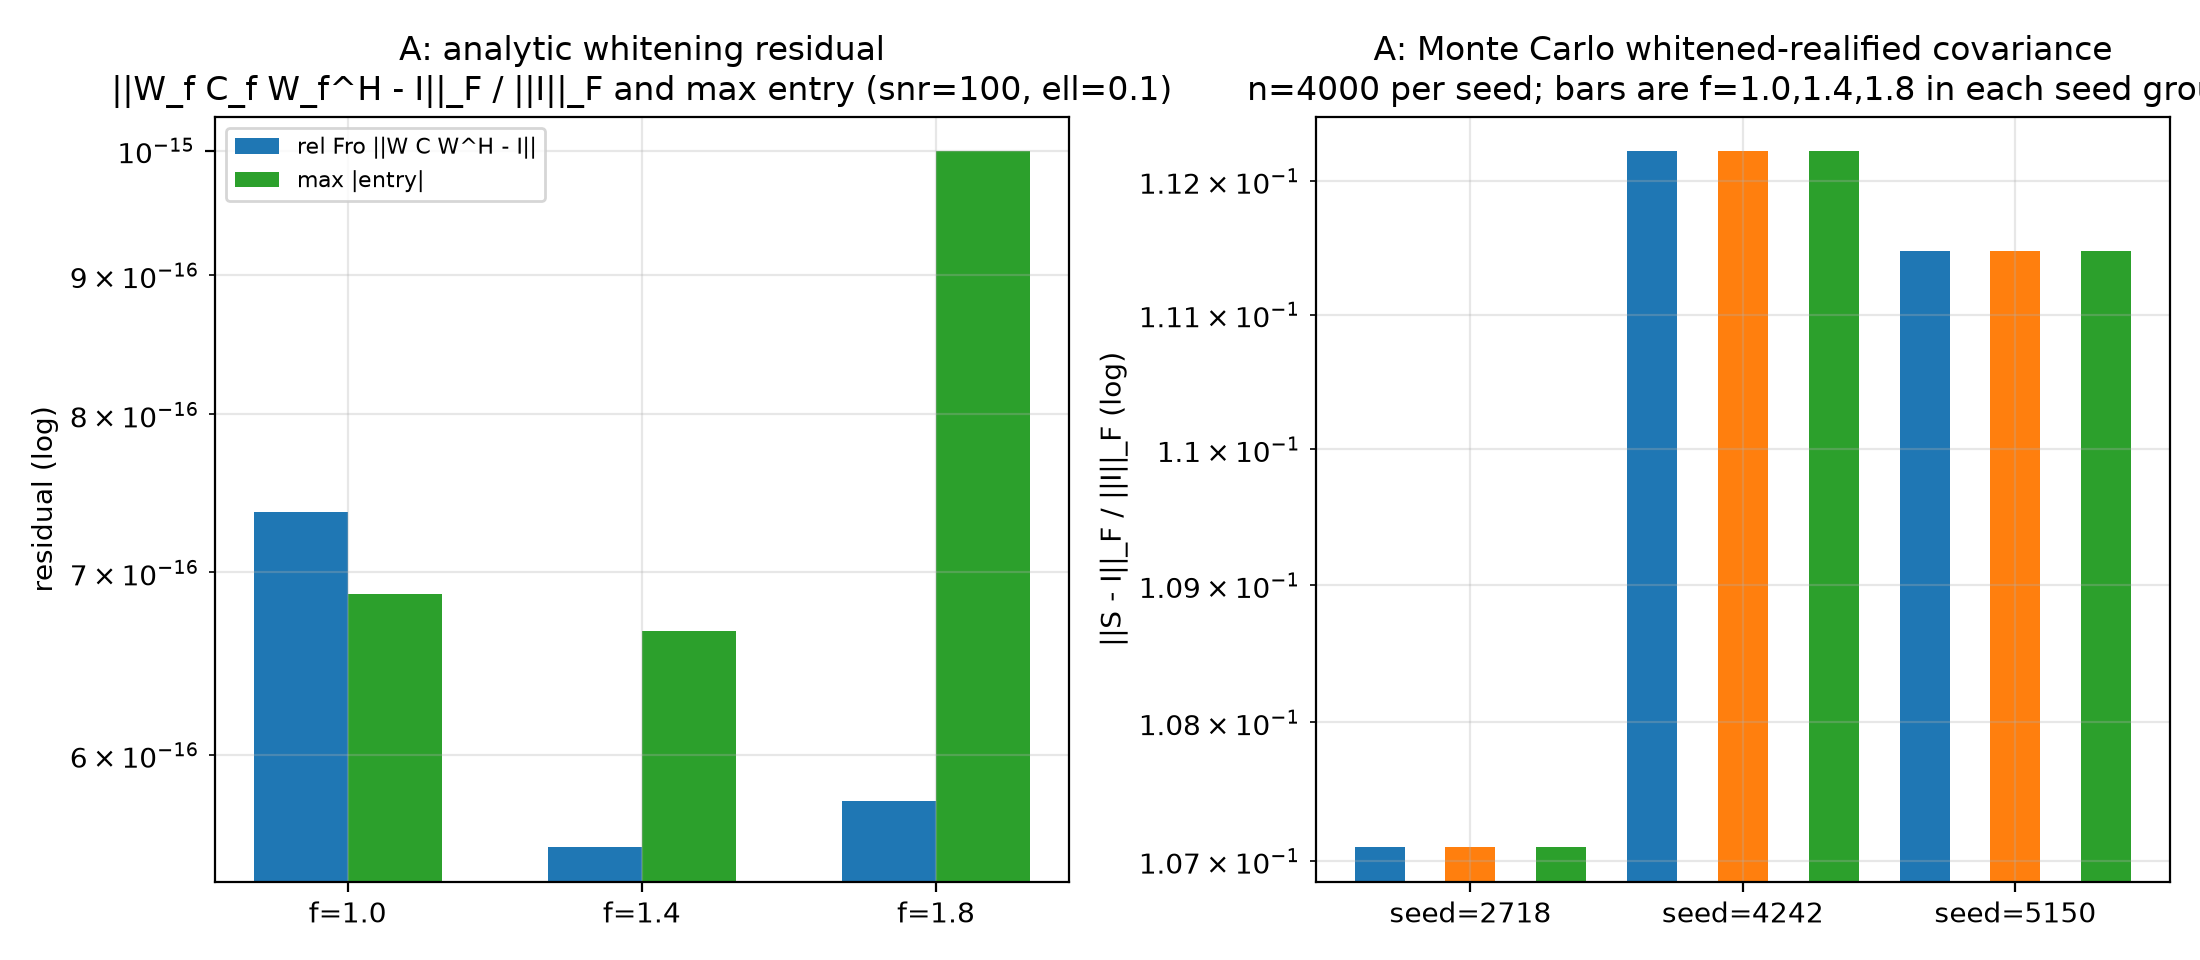
\includegraphics[width=0.86\textwidth]{../figures/family6_noise_whitening_sanity.png}
\caption{Family 6 analytic and Monte-Carlo whitening sanity (recorded).}
\label{fig:f6_sanity}
\end{figure}

\begin{figure}[htbp]
\centering
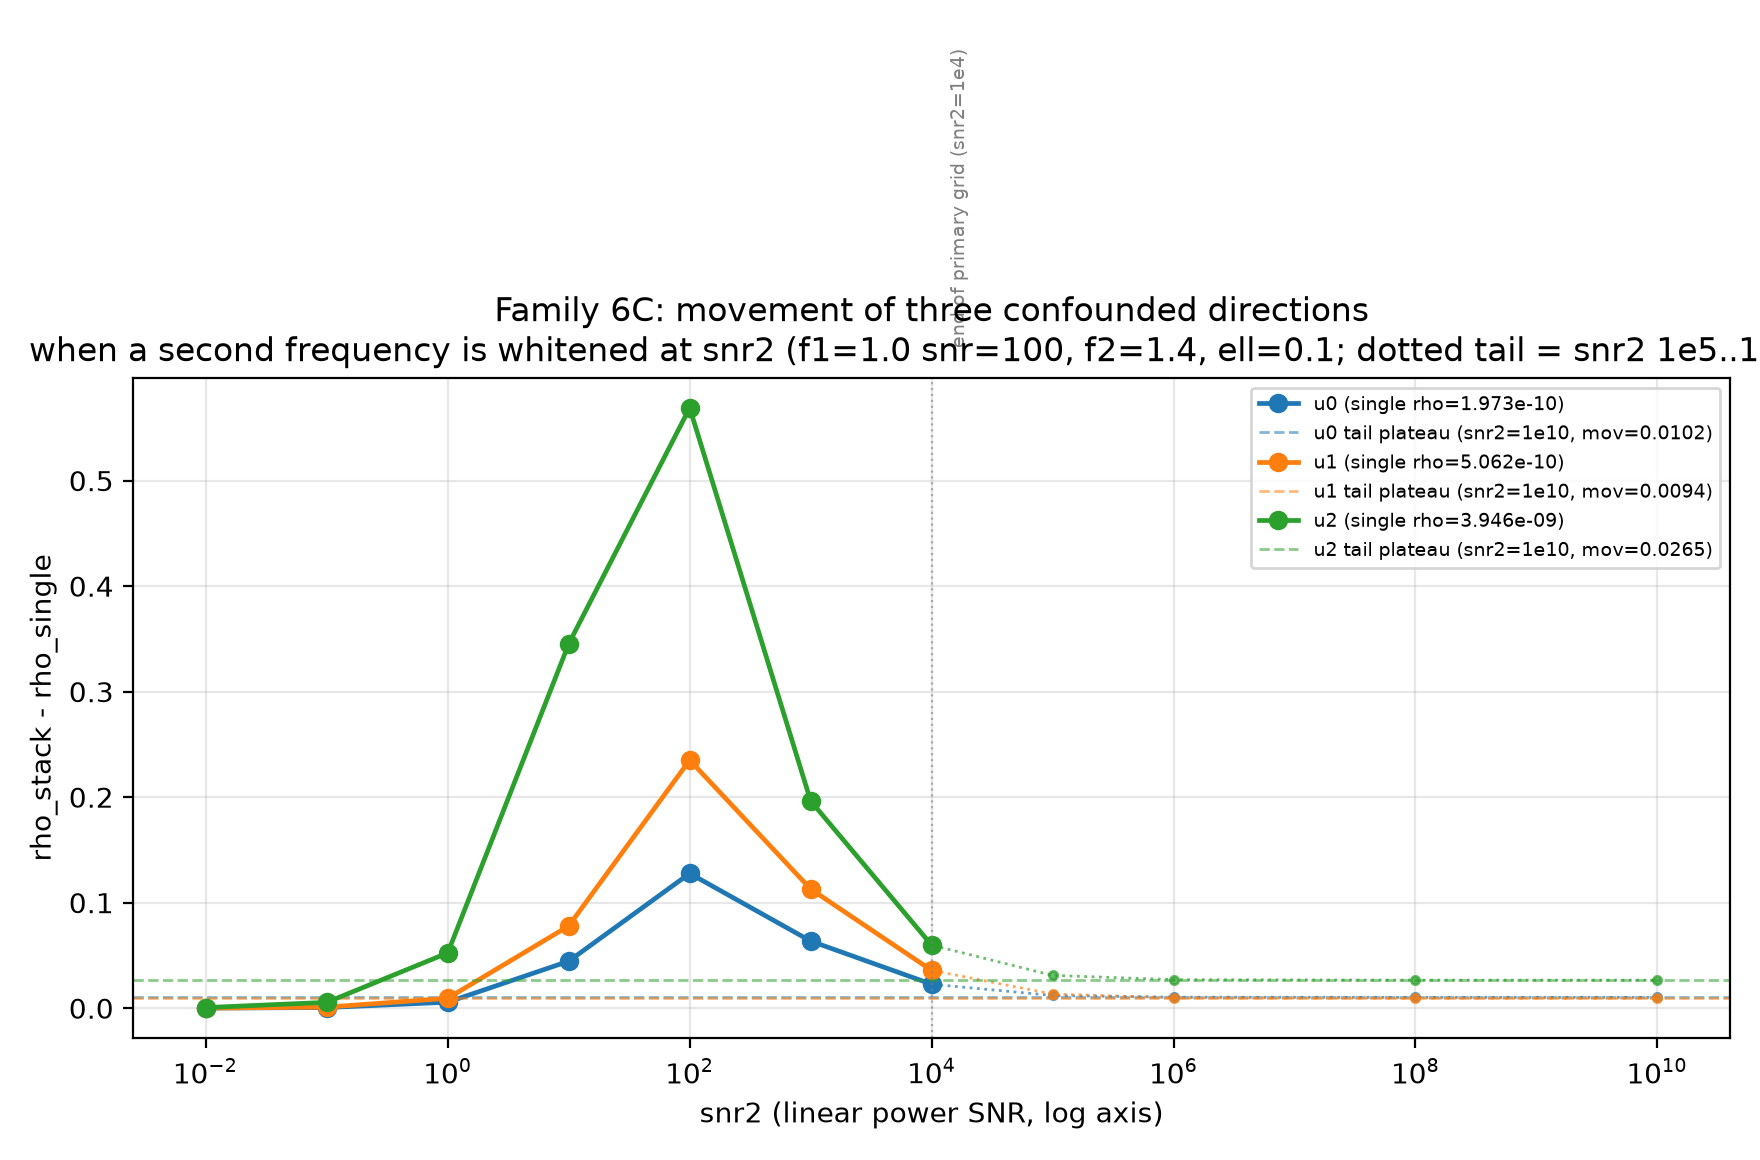
\includegraphics[width=0.86\textwidth]{../figures/family6_snr_sweep.png}
\caption{Family 6 non-monotone SNR movements with a finite high-SNR tail.}
\label{fig:f6_snr}
\end{figure}

\begin{figure}[htbp]
\centering
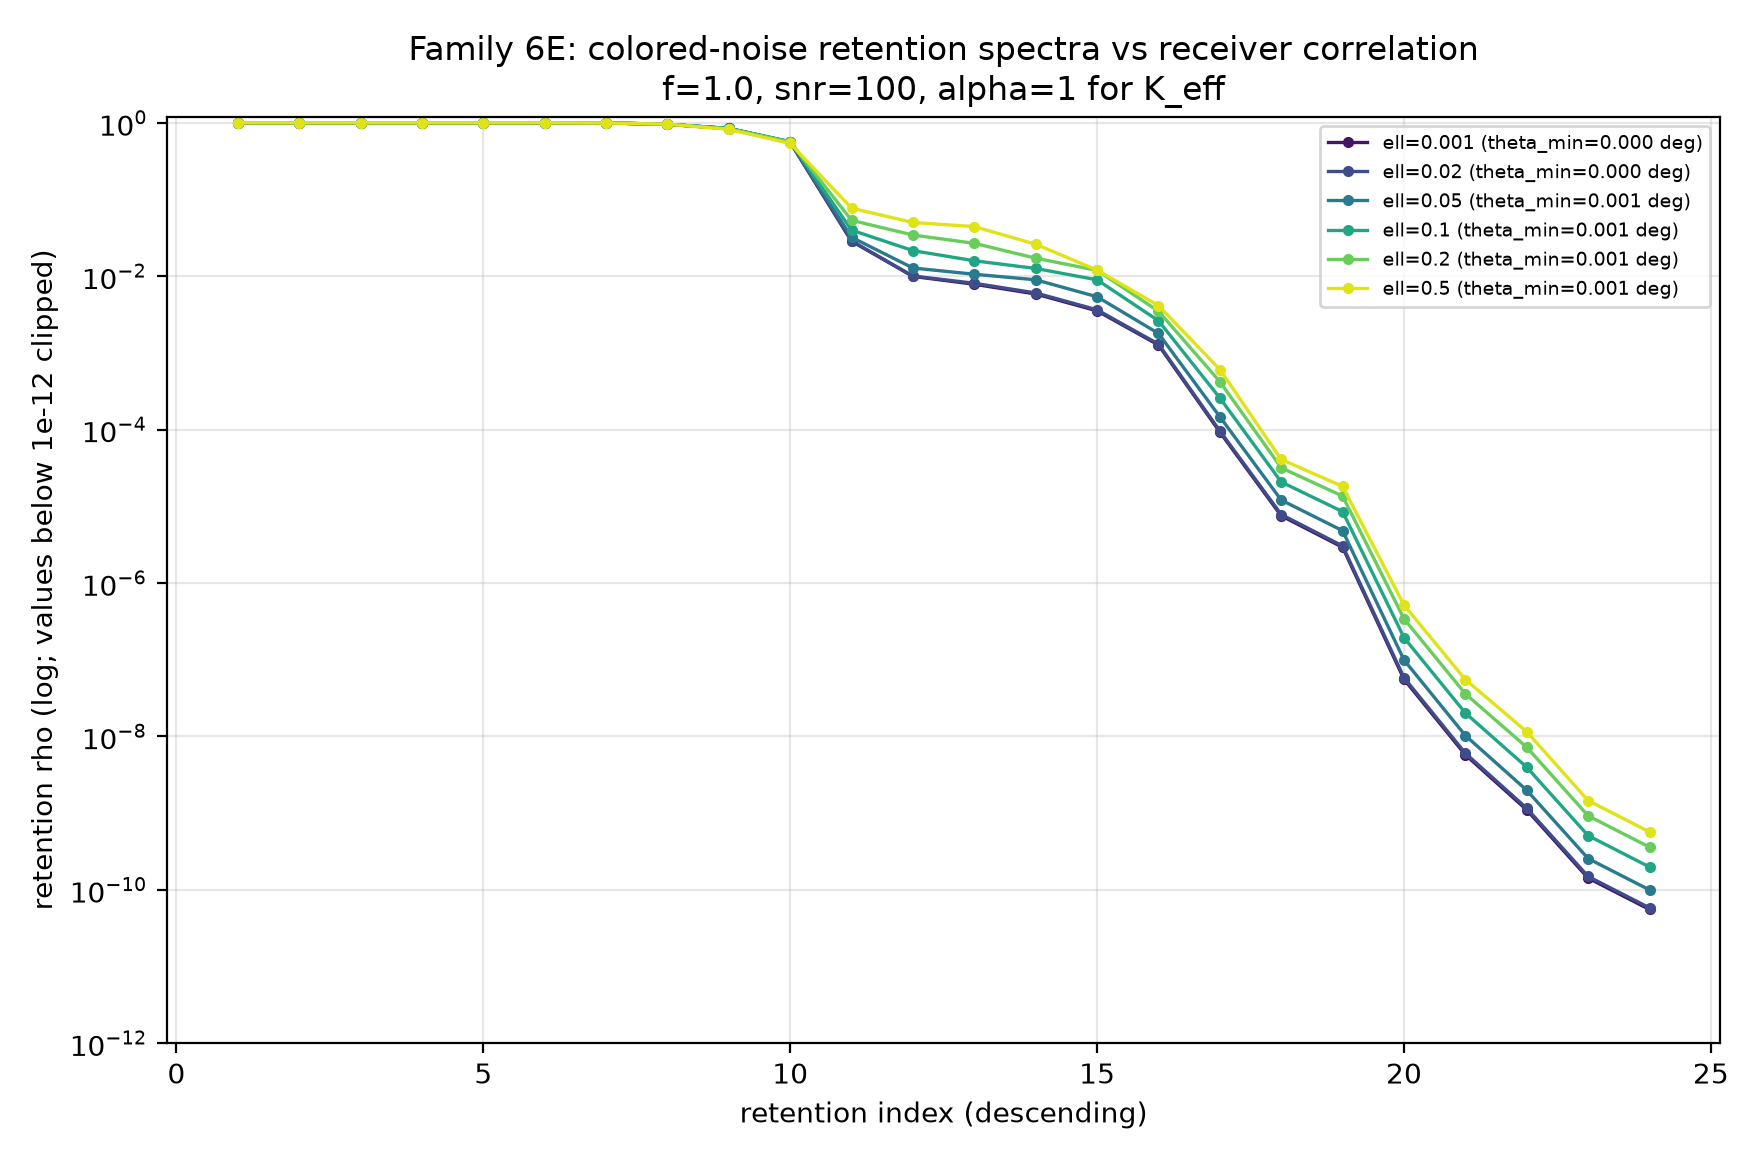
\includegraphics[width=0.86\textwidth]{../figures/family6_correlation_effect.png}
\caption{Family 6 receiver-correlation sweep (recorded, no forced pass).}
\label{fig:f6_corr}
\end{figure}

\begin{figure}[htbp]
\centering
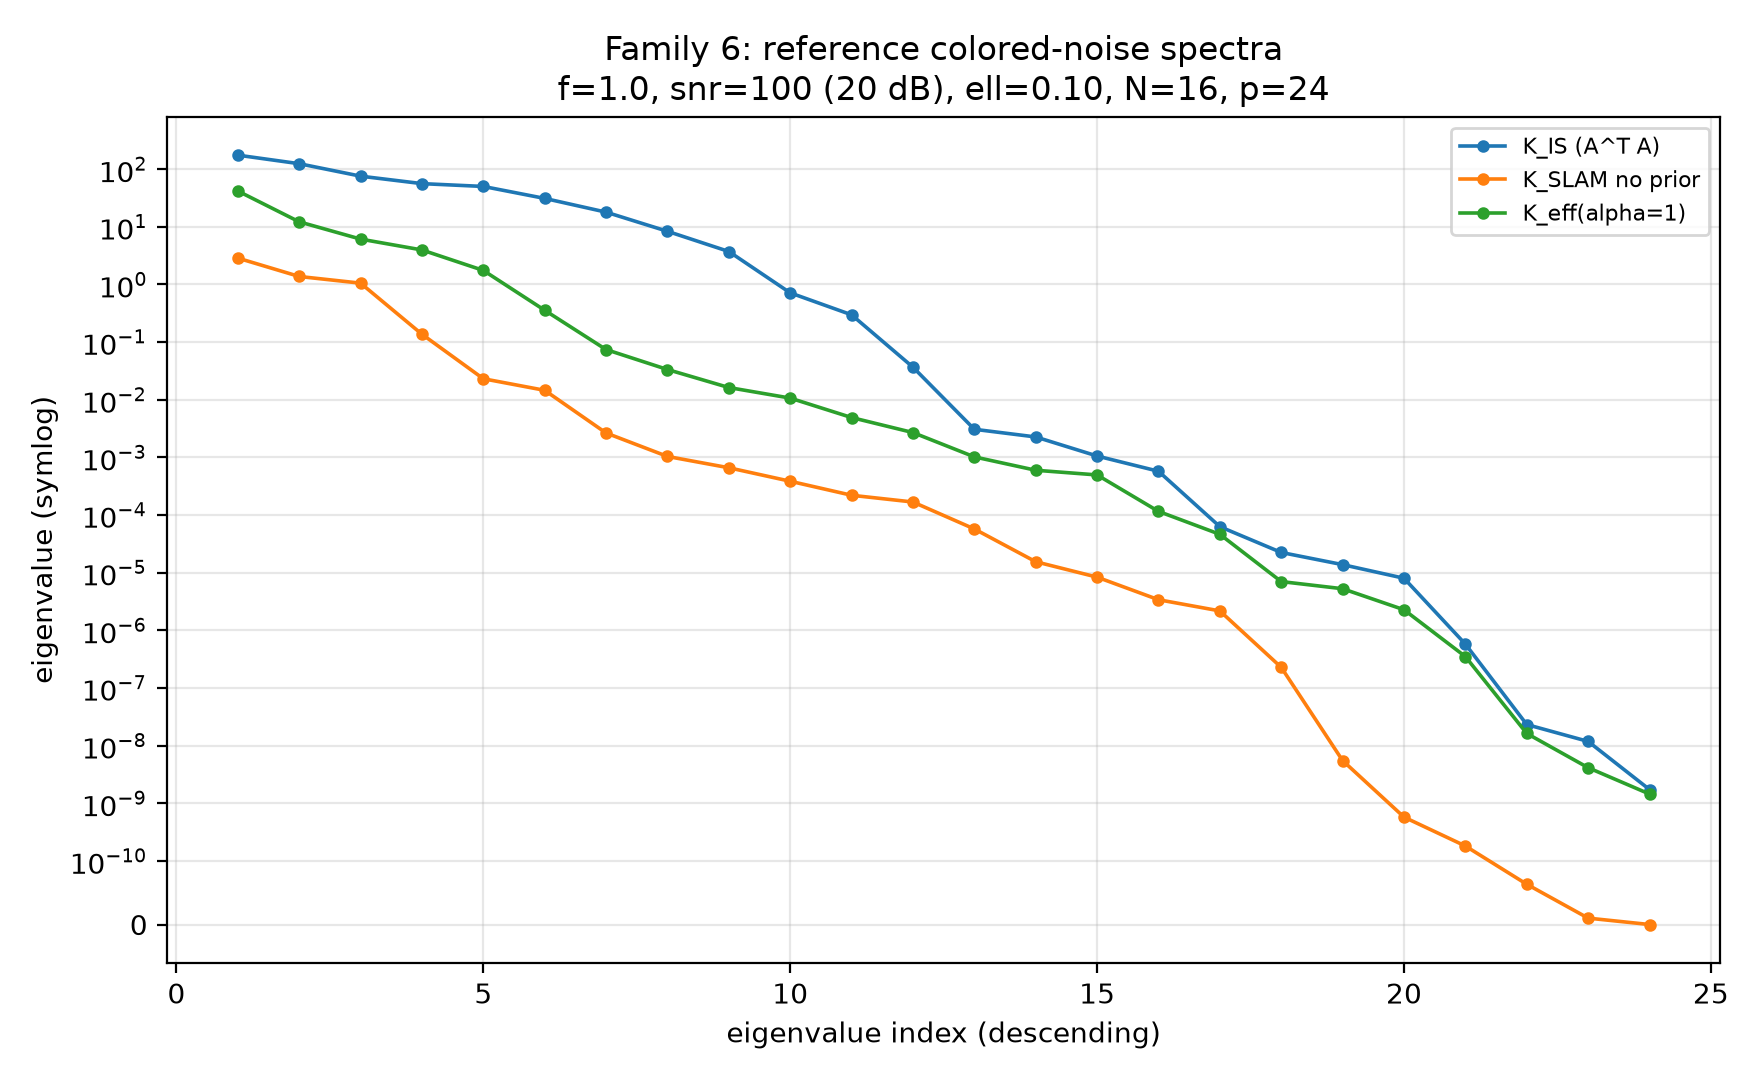
\includegraphics[width=0.86\textwidth]{../figures/family6_retention_spectra_colored.png}
\caption{Family 6 colored-noise retention spectra.}
\label{fig:f6_retention}
\end{figure}

\subsection{Trajectory control under standoff and pose-energy normalization (Family 4c)}\label{sec:family4c}

Family 4c is the Family-4 parent-audit control: curved paths are placed at a
common standoff ($R=1.6$) and each pose's realified $A$-block rows are scaled,
together with the corresponding $B$-block rows, so every pose has unit total
$A$-block Frobenius energy. Normalization is verified after the fact:
$\max|1-\|A_{\mathrm{block}}\|_F|\le2.220\times10^{-16}$ across all tested
trajectories \FDL{} (all five pass the $10^{-12}$ gate). Per-pose
normalization is a declared gain control on the linearized blocks; it does
not prescribe a physical noise covariance.

\begin{table}[htbp]
\centering
\small
\caption{Family 4c retained/confusable mass (raw and normalized;
\texttt{results/family4c\_trajectory\_control.json}).}
\label{tab:f4c}
\begin{tabular}{l l l l l}
\toprule
trajectory & retained (raw) & retained (norm.) &
confusable (raw) & confusable (norm.) \\
\midrule
straight\_same\_mid & 8.353517 & 8.269820 & 15.646483 & 15.730180 \\
arc90\_same\_standoff & 9.407162 & 9.408661 & 14.592838 & 14.591339 \\
arc180\_same\_standoff & 7.999302 & 7.997790 & 16.000698 & 16.002210 \\
arc270\_same\_standoff & 7.536362 & 7.535343 & 16.463638 & 16.464657 \\
circle360\_same\_standoff & 7.703633 & 7.701223 & 16.296367 & 16.298777 \\
\bottomrule
\end{tabular}
\end{table}

The raw and normalized orderings do not flip \OBS{}: retained mass descends as
arc90 $>$ straight $>$ arc180 $>$ circle360 $>$ arc270 in both columns, and
confusable mass ascends in the same order. The four-core hypothesis
(circle360 $>$ arc180 $>$ arc90 $>$ straight) therefore remains false under
the normalized control: \texttt{hypothesis\_holds\_for\_four\_core=false},
recorded without a forced pass. This preserves the Family 4 trajectory
counterexample \CTX{} under a cleaner geometry control; arc270 is the lowest
retained-mass trajectory in this five-path set. No universal trajectory
ordering is asserted: equal standoff fixes curved-path range but still changes
continuous design length and sampled polyline length with angular coverage,
and the straight path still varies standoff \OBS{}.

\begin{figure}[htbp]
\centering
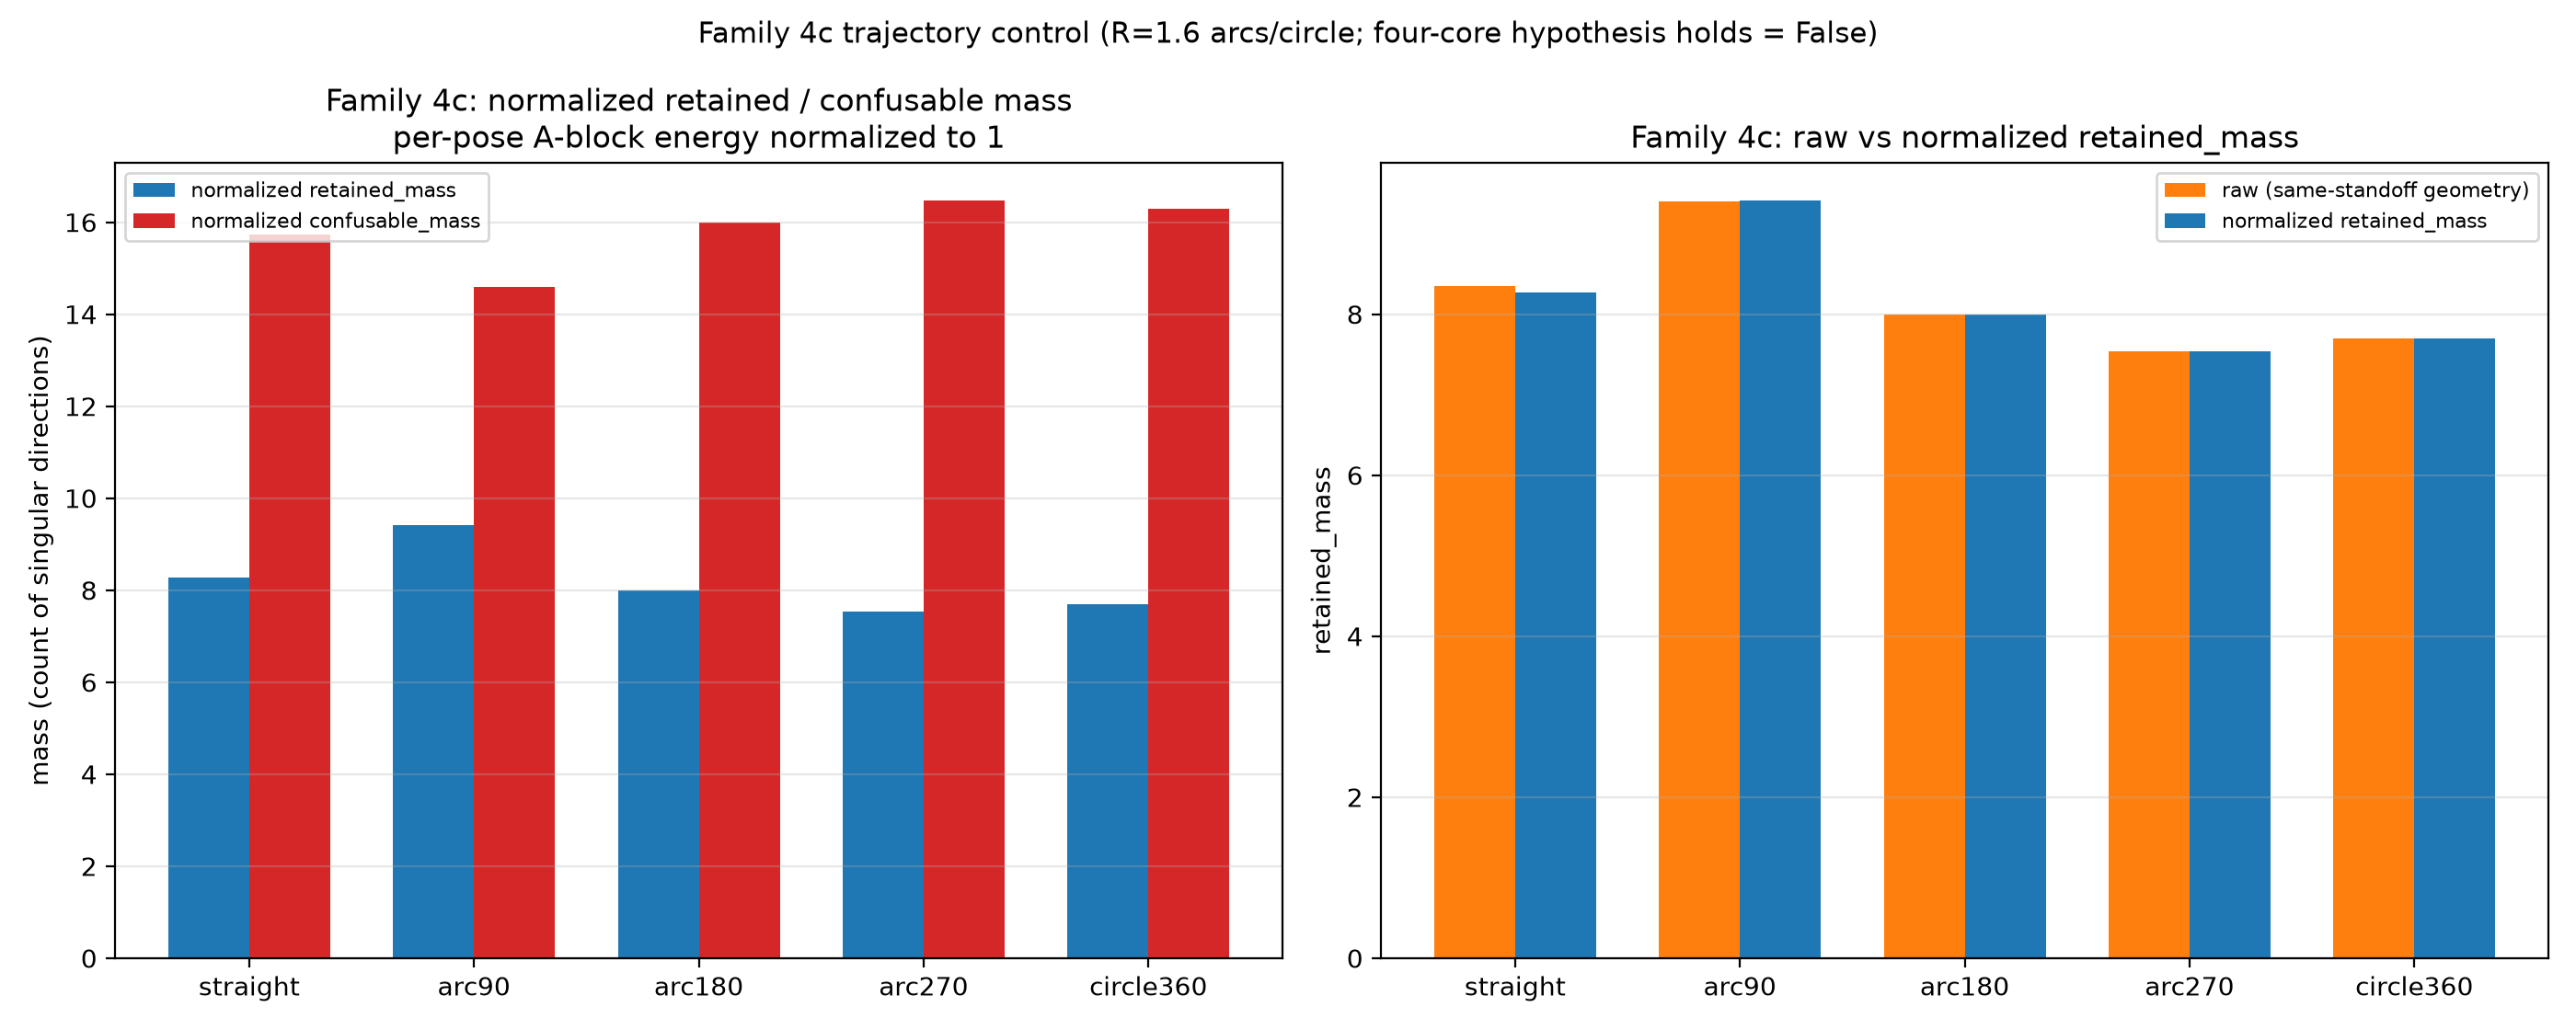
\includegraphics[width=0.86\textwidth]{../figures/family4c_trajectory_control.png}
\caption{Family 4c same-standoff raw and normalized trajectory control.}
\label{fig:f4c}
\end{figure}

\subsection{Resolution, rank events, and stable-transversality diagnostics (Family 7)}\label{sec:family7}

Family 7 is a new finite-grid diagnostic family: for every resolution $N$ the
same continuous two-blob scene is sampled on that grid and the smooth p=24
basis is rebuilt, and separate frequency and contrast sweeps are recorded at
N=16. These are diagnostics on the executed grids, explicitly not continuum
or transversality proofs \OBS{}.

\begin{table}[htbp]
\centering
\small
\caption{Family 7 key numbers by resolution
(\texttt{results/family7\_refinement\_rank.json}).}
\label{tab:f7}
\begin{tabular}{l l}
\toprule
quantity & value \\
\midrule
ranks at N=16/24/32/40/48 & $r_A=24$, $r_B=18$, $r_{AB}=42$, $r_{K}=24$;
rank identity true at every computed $N$ \\
$\theta_{\min}$ (deg), N=16 to 48 &
$4.253070\times10^{-4}$ to $4.188332\times10^{-4}$ (monotone decreasing,
span $6.474\times10^{-6}$ deg) \\
near-confounded directions (cos$^2>1-10^{-8}$) &
$[4,4,4,4,4]$; constant over the tested grid \\
frequency sweep (21 points, f=0.6..2.6) &
rank events 0; 21 literal near-crossing flags, all on the lowest
numerical near-null $K_{\mathrm{eff}}$ pairs \\
$s=0$ Born gates &
B/A Fro ratio 0.0; rel.\ Fro $K_{\mathrm{SLAM}}-K_{\mathrm{IS}}$ 0.0
(both pass $<10^{-12}$) \\
Born/full rel.\ Fro discrepancy &
$1.894\times10^{-3}$ at $s=0.01$ growing to $0.1975$ at $s=1$ \\
contrast rank transition & expected $s=0\to0.01$ exit
($r_B:0\to18$, $r_{AB}:24\to42$), recorded as an observed machine-rank event \\
\bottomrule
\end{tabular}
\end{table}

Across N=16..48 the machine ranks remain constant and the rank identity passes
for every computed row \FDL{}. The minimum principal angle
$\theta_{\min}$ decreases monotonically on the tested grid
($4.253070\times10^{-4}$ to $4.188332\times10^{-4}$ deg), and the number of
near-confounded directions is constant at 4 \OBS{}. In the frequency sweep no
rank event occurs, but every one of the 21 sweep points satisfies the literal
smallest-gap near-crossing inequality on one of the lowest ascending pairs
([0,1] or [1,2]); those flags sit in the repeated numerical near-null tail of
$K_{\mathrm{eff}}$ and are recorded as the literal criterion, not as certified
eigenvalue crossings or transversality failures. The $s=0$ Born gates pass
exactly \FDL{} ($B=0$ and $K_{\mathrm{SLAM}}=K_{\mathrm{IS}}$ to the declared
$10^{-12}$ relative gate), while the Born/full-wave discrepancy grows from
$1.894\times10^{-3}$ at $s=0.01$ to $0.1975$ at $s=1$ \OBS{}. No forced pass
is applied anywhere in Family 7.

\begin{figure}[htbp]
\centering
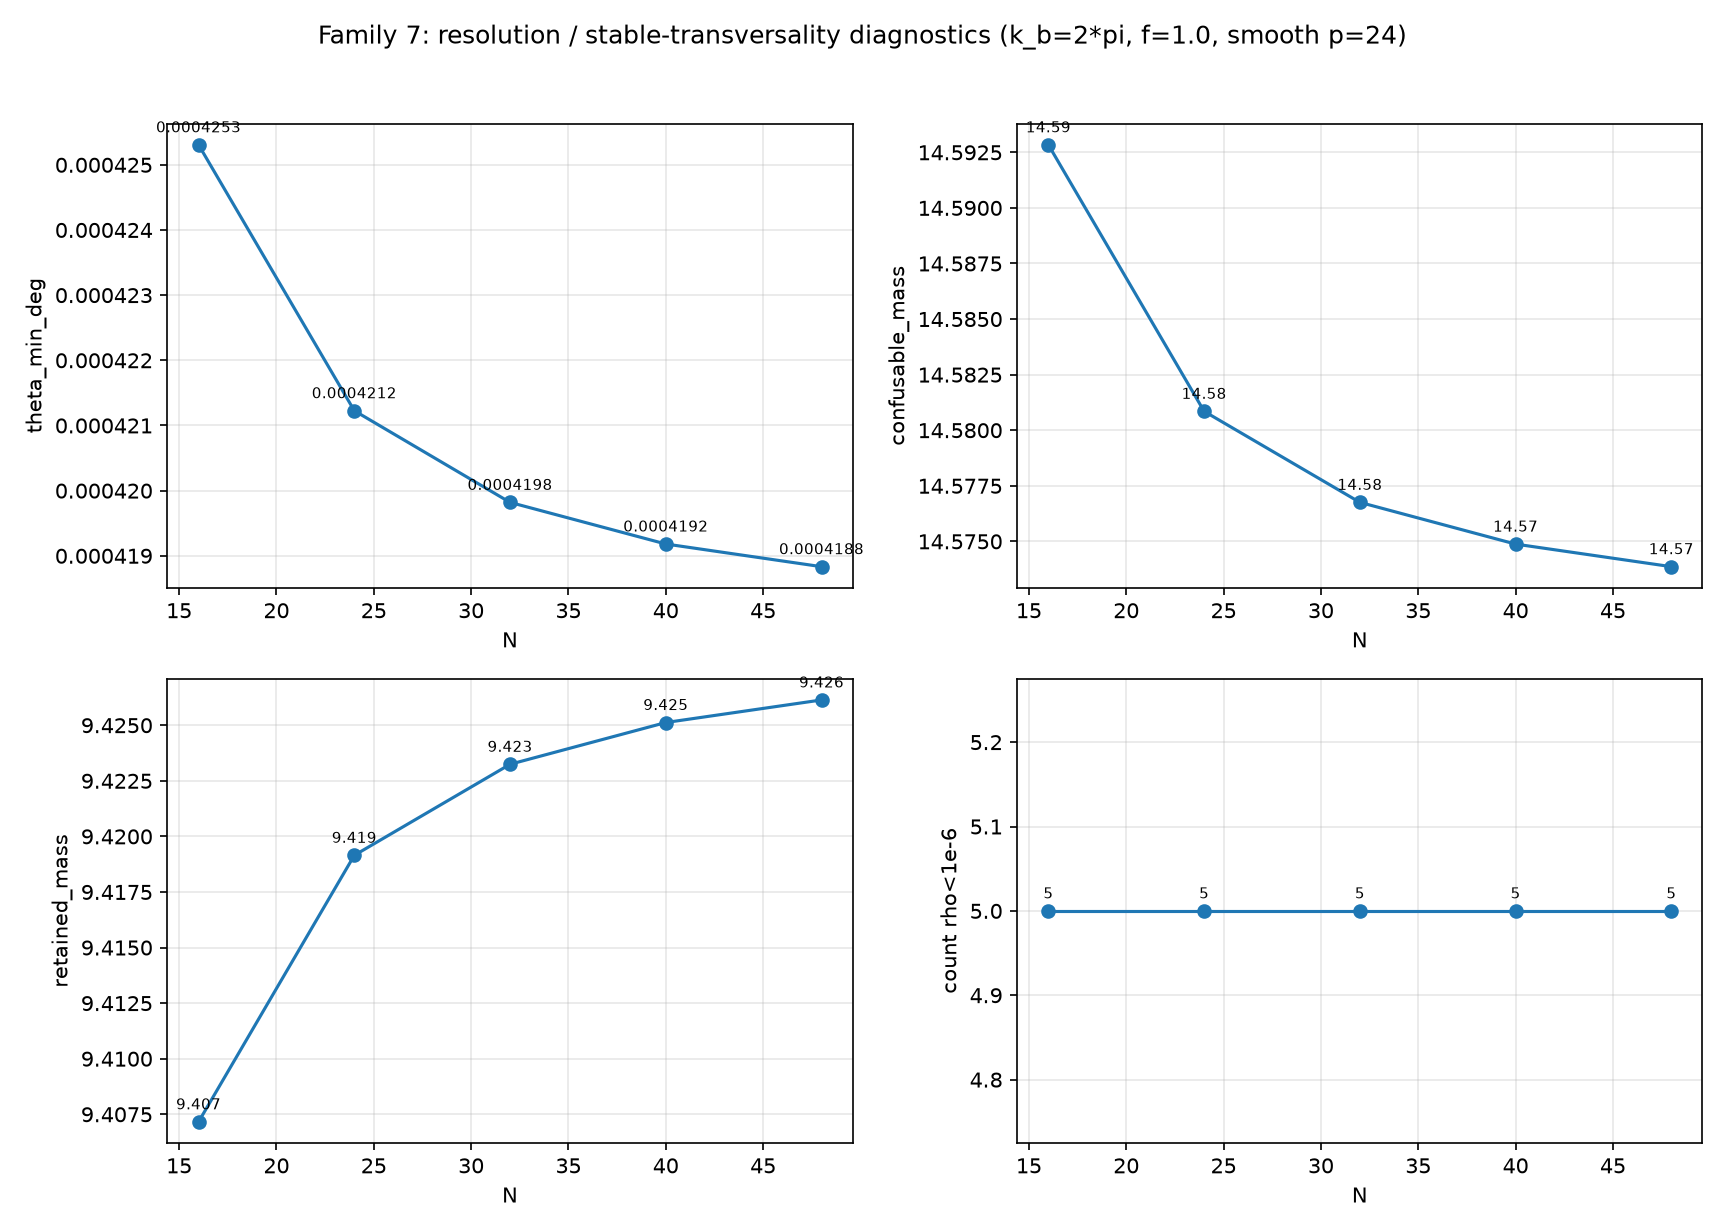
\includegraphics[width=0.86\textwidth]{../figures/family7_resolution_convergence.png}
\caption{Family 7 resolution convergence of $\theta_{\min}$ and spectral masses.}
\label{fig:f7_resolution}
\end{figure}

\begin{figure}[htbp]
\centering
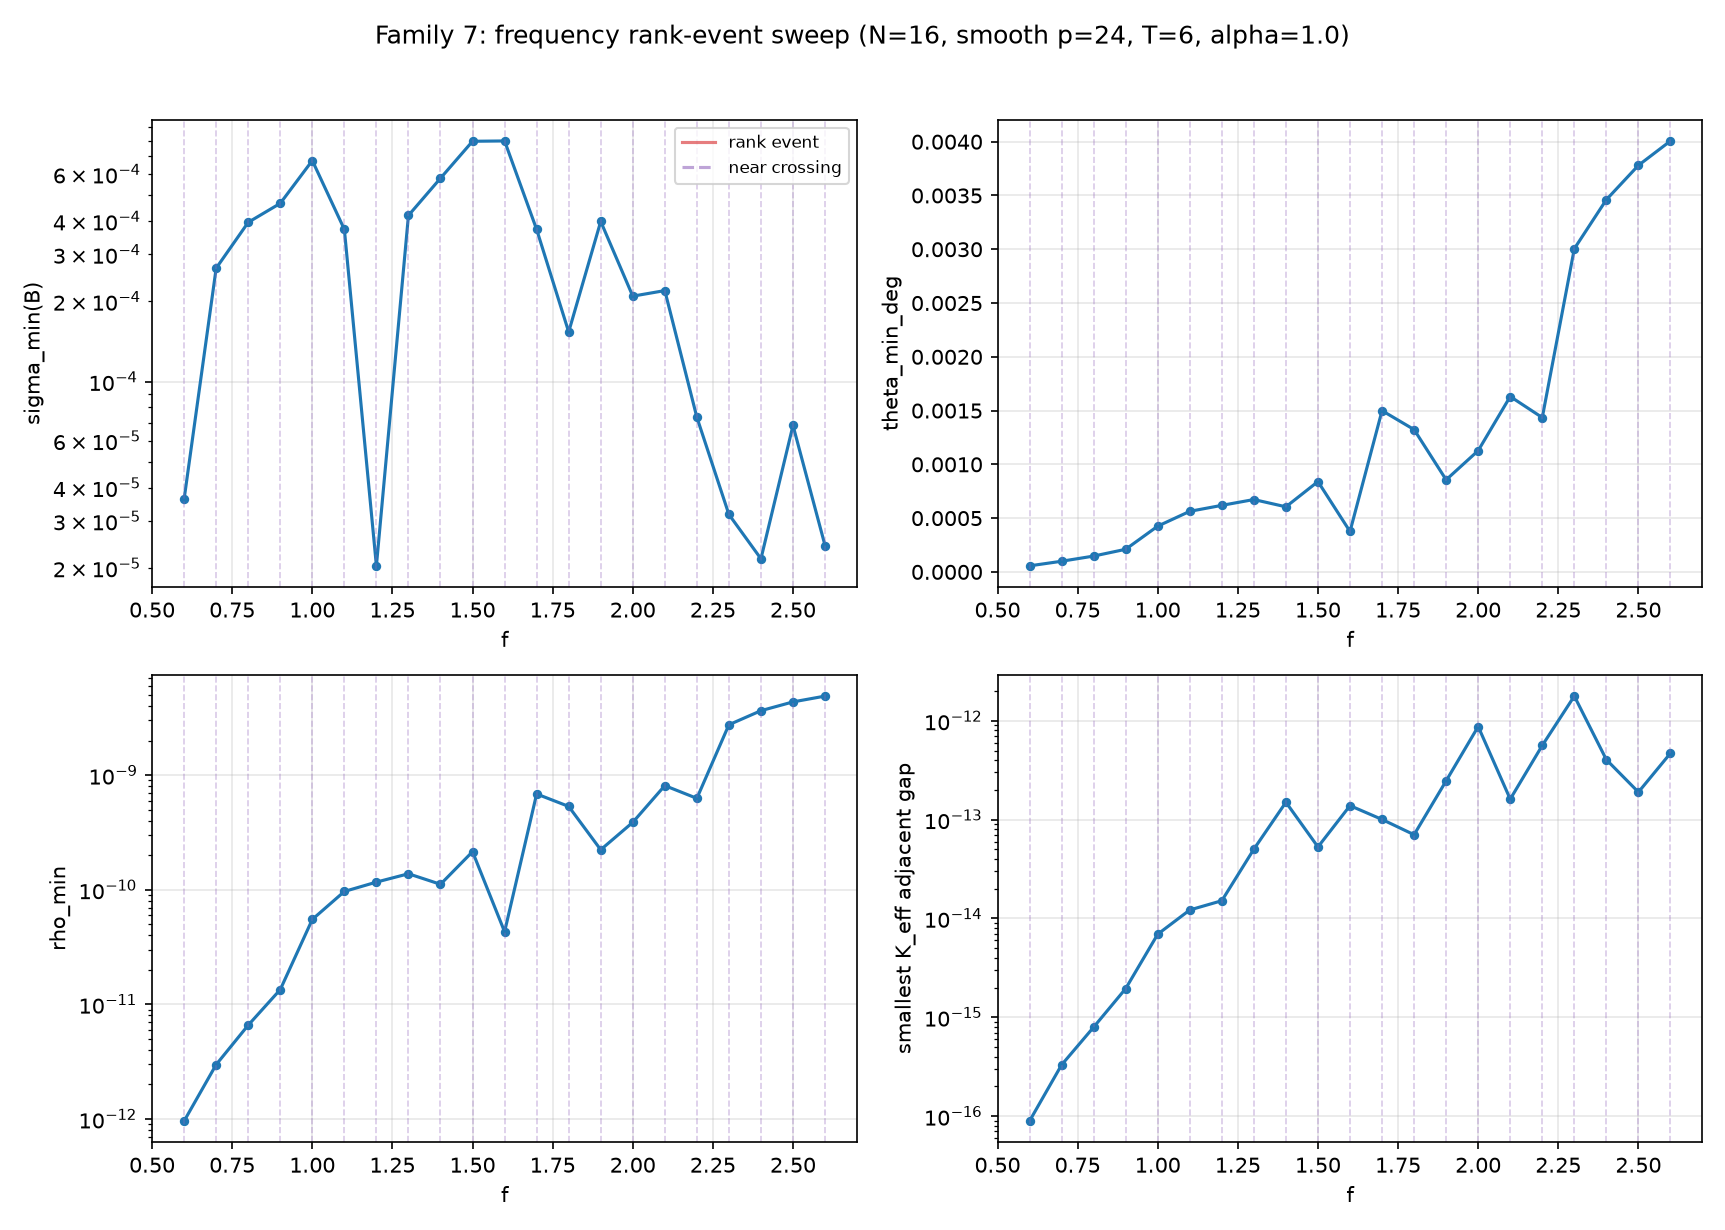
\includegraphics[width=0.86\textwidth]{../figures/family7_frequency_rank_sweep.png}
\caption{Family 7 frequency rank-event and near-crossing sweep.}
\label{fig:f7_frequency}
\end{figure}

\begin{figure}[htbp]
\centering
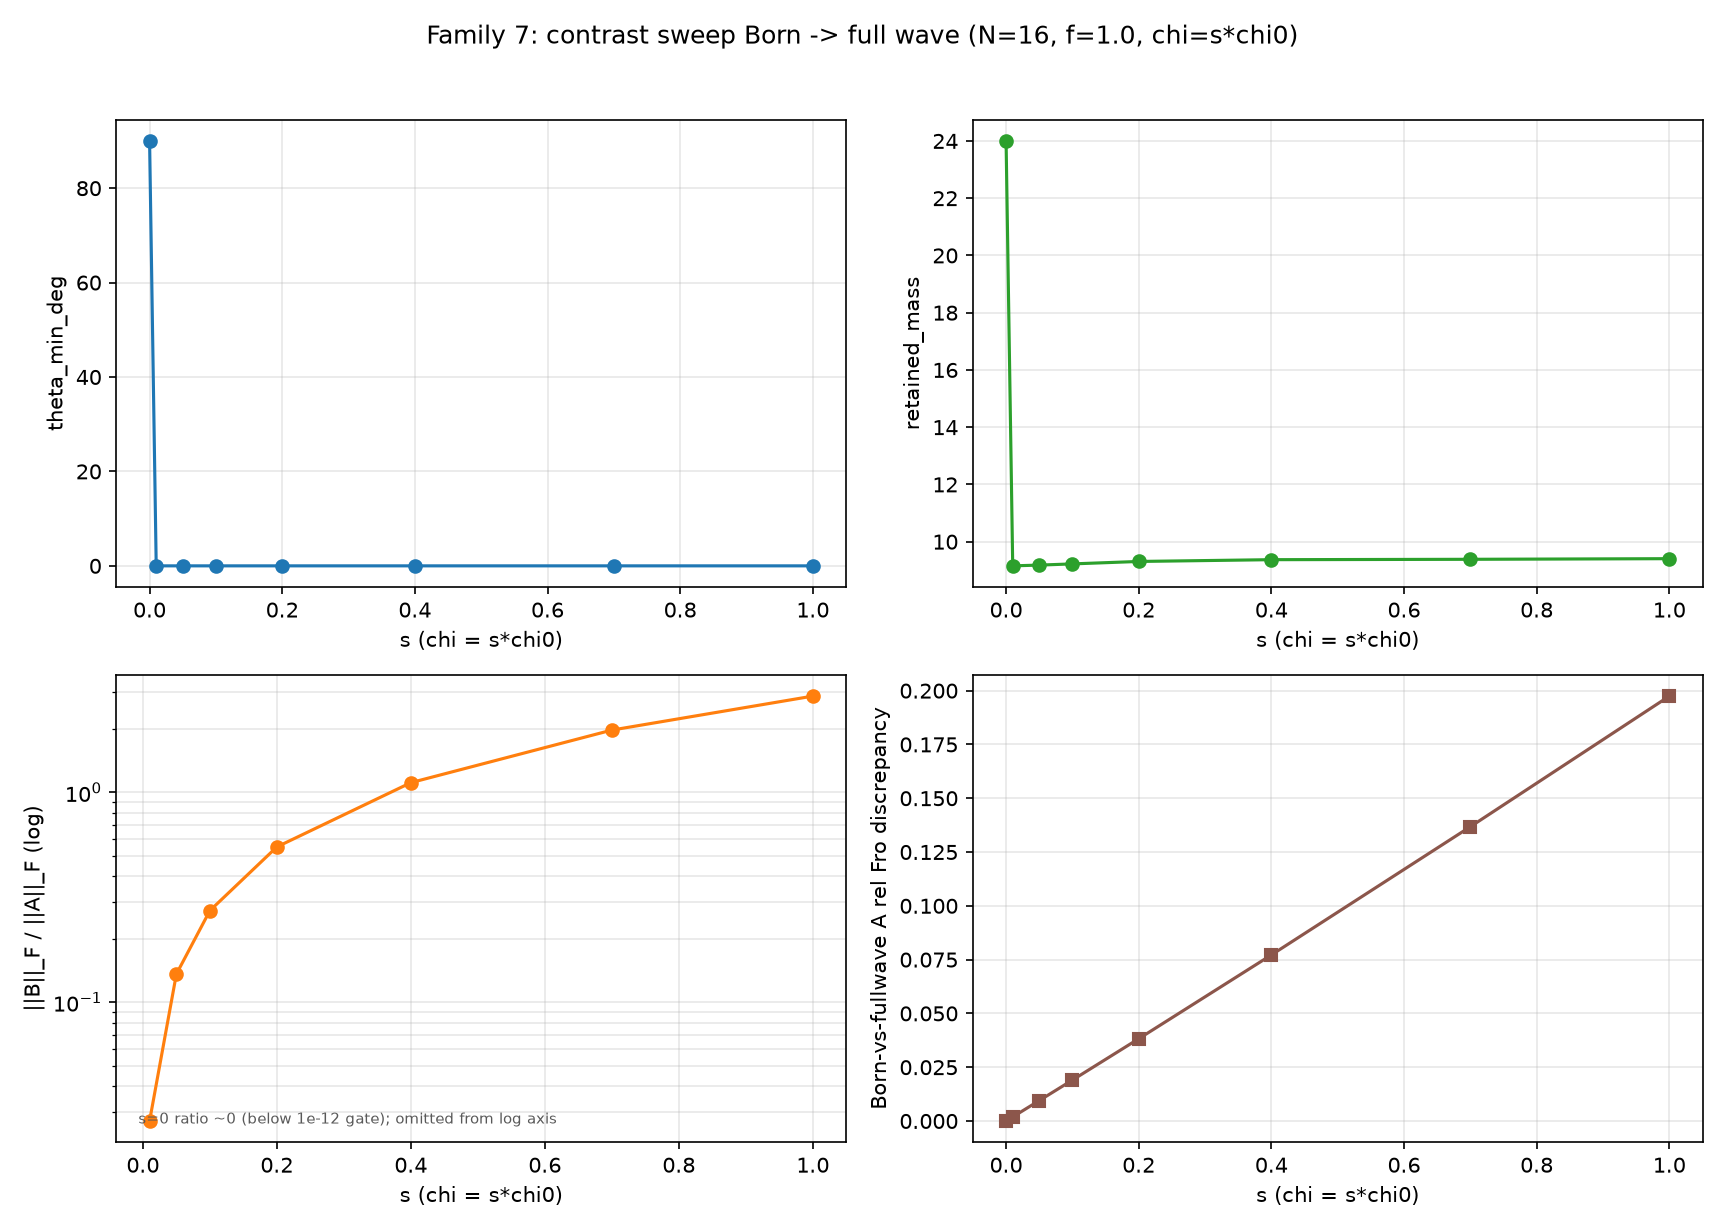
\includegraphics[width=0.86\textwidth]{../figures/family7_contrast_sweep.png}
\caption{Family 7 Born-to-full-wave contrast sweep.}
\label{fig:f7_contrast}
\end{figure}

\subsection{Current-space $G_S$/SOM vs map-tangent $A/K_{\mathrm{eff}}$ distinction (Family 8)}\label{sec:family8}

Family 8 makes the current-space sensing map $G_S$ (stacked over poses) and
the map-tangent Jacobian $A_c$/pixel kernel $K_{\mathrm{eff}}$ explicit in the
same $N^2$ pixel space, at N=16, T=6, f=1.0, with $\alpha=1.0$.

\begin{table}[htbp]
\centering
\small
\caption{Family 8 key numbers
(\texttt{results/family8\_som\_distinction.json}).}
\label{tab:f8}
\begin{tabular}{l l}
\toprule
quantity & value \\
\midrule
full-wave composition stack rel.\ Fro &
0 (identical float path; per-pose 0) \\
Born composition stack rel.\ Fro & $7.05442\times10^{-17}$ \\
Range$(A_c)\subseteq$Range$(G_S)$ &
projector difference $3.5260\times10^{-15}$; containment residual
$2.3354\times10^{-15}$; ranks 24 $\le$ 24 \\
literal arccos angle (U subspaces) &
$2.1073\times10^{-8}$ rad, the $\sqrt{2\epsilon}$ roundoff floor;
literal rad gate false \\
right-subspace principal angles $V_{GS}$ vs $V_A$ &
count $<10^{-8}$ deg: 0/24; median $29.70670$ deg; max $89.79380$ deg; \\
 & min $0.46609$ deg; row-proj diff 0.999994 \\
$K_{\mathrm{eff}}$ confounded-vector overlaps &
max squared overlaps with $V_{GS}$: $3.2680\times10^{-3}$; \\
 & with $V_A$: $5.7556\times10^{-8}$ \\
mode counts at rel.\ thresholds $10^{-6}$/$10^{-3}$ &
$\sigma(G_S)$ [13, 8]; $\sigma(A_c)$ [23, 12]; \\
 & $\sigma(A_R)$ [46, 23]; eig$(K_{\mathrm{IS}})$ [23, 12] \\
\bottomrule
\end{tabular}
\end{table}

The full-wave composition identity is bit-identical (stack relative Frobenius
0), and the Born composition identity holds to $7.054\times10^{-17}$
\FDL{}. Range containment of $A_c$ in $G_S$ holds machine-exactly on the
tested full-rank data space (projector difference $3.526\times10^{-15}$ and
containment residual $2.335\times10^{-15}$) \FDL{}; the recorded arccos angle
sits at the roundoff floor for identical full-rank subspaces, so the direct
O($\epsilon$) projector/residual checks are the meaningful gates. By contrast,
the right singular pixel-mode subspaces $V_{GS}$ and $V_A$ are strongly
distinct \OBS{}: zero of 24 principal angles fall below $10^{-8}$ deg, the
median is $29.70670$ deg, the maximum is $89.79380$ deg, and the row-space
projector difference is 0.999994 (nearly orthogonal). The three most
confounded $K_{\mathrm{eff}}$ directions are nearly orthogonal to both mode
sets on the tested scenario: their maximum squared overlaps are about
$3\times10^{-3}$ with $V_{GS}$ and only about $6\times10^{-8}$ with $V_A$.
Mode counts also differ once the different threshold scales are recorded
side by side (SOM count vs map-information count), and no SOM quality claim
is made.

\begin{figure}[htbp]
\centering
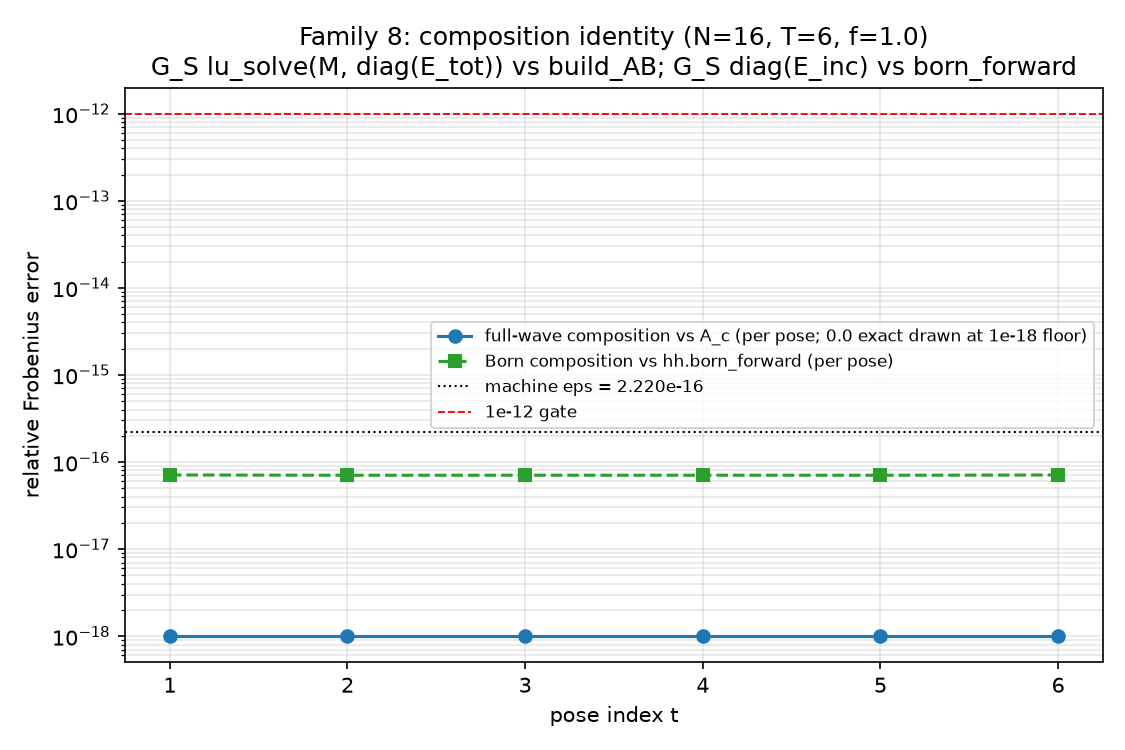
\includegraphics[width=0.86\textwidth]{../figures/family8_composition_identity.png}
\caption{Family 8 per-pose full-wave and Born composition identities.}
\label{fig:f8_composition}
\end{figure}

\begin{figure}[htbp]
\centering
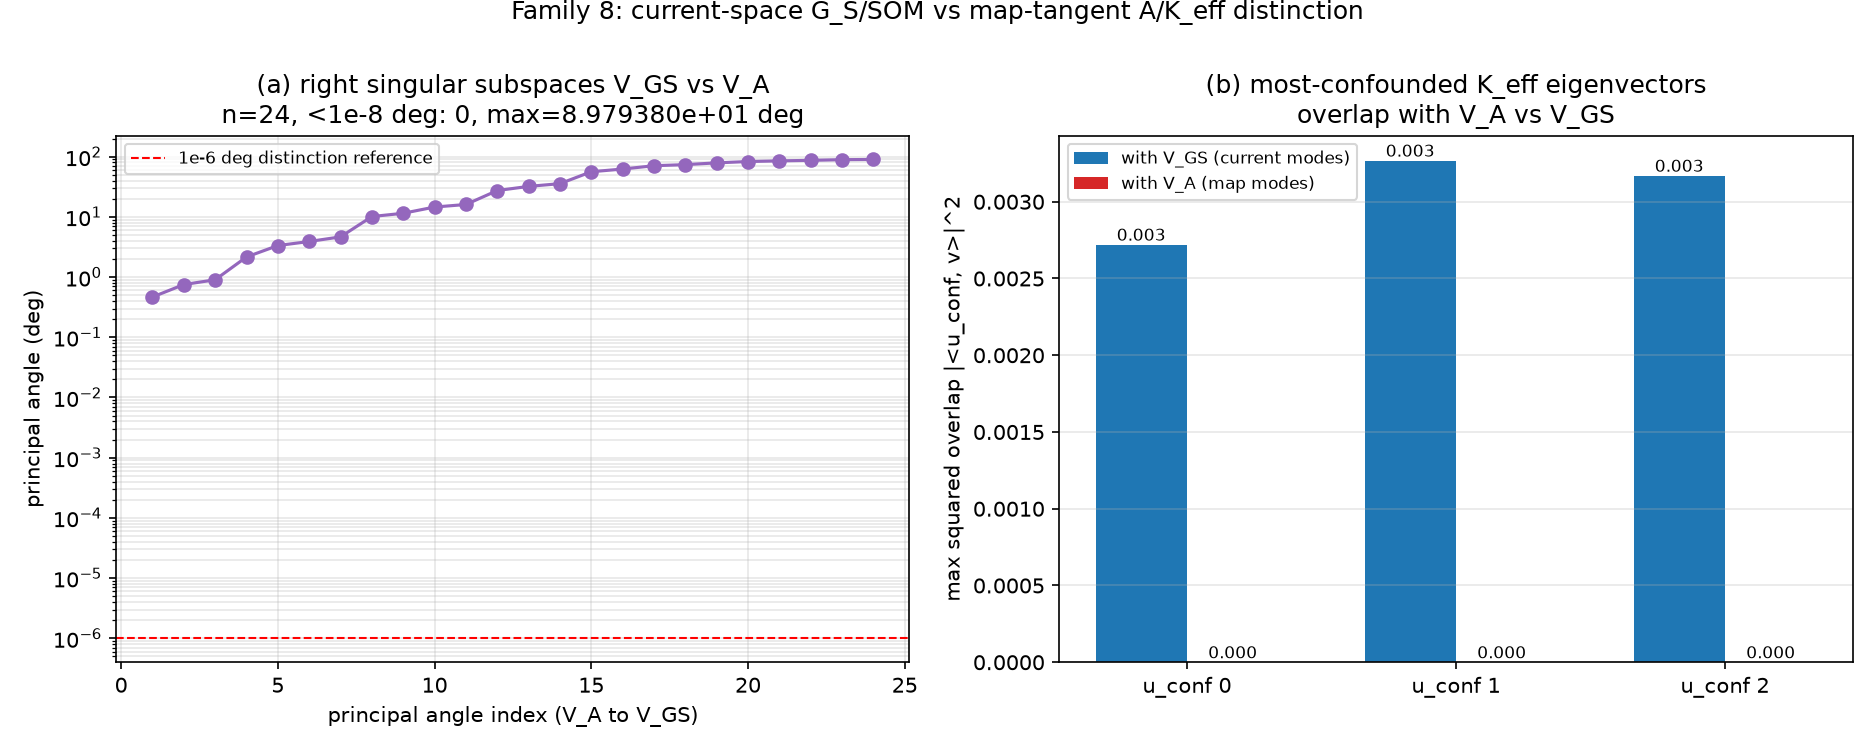
\includegraphics[width=0.86\textwidth]{../figures/family8_mode_distinction.png}
\caption{Family 8 principal-angle and overlap distinction between
$V_{GS}$/SOM and $V_A$/$K_{\mathrm{eff}}$ mode families.}
\label{fig:f8_modes}
\end{figure}

\subsection{Seed replications and component ablations (Family 9)}\label{sec:family9}

Family 9 reruns the deterministic Family 2 (c1--c3) and Family 4 check-C
claims over seven scenes (five 8-blob seeds 1001--1005 rescaled to the
two-blob norm, the standard two-blob scene, and a ring scene) and records
descriptive component ablations.

\begin{table}[htbp]
\centering
\small
\caption{Family 9 replication and ablation key numbers
(\texttt{results/family9\_replications\_ablation.json}).}
\label{tab:f9}
\begin{tabular}{l l}
\toprule
quantity & value \\
\midrule
rank identity over 7 scenes & 6/7; ring residual 1 (machine-rank boundary) \\
no-prior retention identity & 7/7 (max diff $2.817\times10^{-15}$;
typical $\sim10^{-15}$) \\
kernel identity & F2 subspace gate 7/7; identity support 6/7;
nullity match 6/7 (ring mismatch) \\
frequency diversity & 7/7; 3/3 directions moved above $10^{-4}$ on every scene \\
pose-DOF retained mass & known 24.000; x-only 18.020; y-only 18.029;
$\theta$-only 21.362; \\
 & xy 12.573; full 9.407 \\
receiver-count retained mass ($n_{\mathrm{rx}}$=1/2/4/8) &
0 / 6.000 / 9.407 / 9.399 (mixed-$r_A$ rows; not a pure effect) \\
pose-count retained mass (T=3/6/12) &
15.000 / 9.407 / 6.579 (monotone on this grid) \\
basis retained mass (p=12/24/36) &
0.157 / 9.407 / 18.750 (fixed $B$ adds $A$ directions) \\
\bottomrule
\end{tabular}
\end{table}

The replication record is \FDL{} on the executed scenes where the gates pass,
with one preserved boundary event: the ring scene's smallest
$K_{\mathrm{SLAM}}$ eigenvalue falls below the family-2 eig rank tolerance
while $C=(I-ZZ^T)A_s$ remains full rank at its own SVD tolerance, so the
literal machine-rank identity records residual 1 and nullity mismatch.
That ring row is a recorded machine-rank boundary, not evidence against the
exact algebraic identity \OBS{}. Retention and frequency diversity pass on
all seven scenes. The ablations are descriptive, with no forced pass:
$\theta$-only nuisance destroys less retained mass than the translational
DOFs, receiver-count rows mix changing $r_A$ with receiver count and are not
interpreted as a pure effect, pose-count retention declines monotonically on
the tested T grid as more nuisance columns are added, and basis-p retention
grows with $r_A$ for a fixed $B$. No universal claim is drawn from these
single-geometry trends.

\begin{figure}[htbp]
\centering
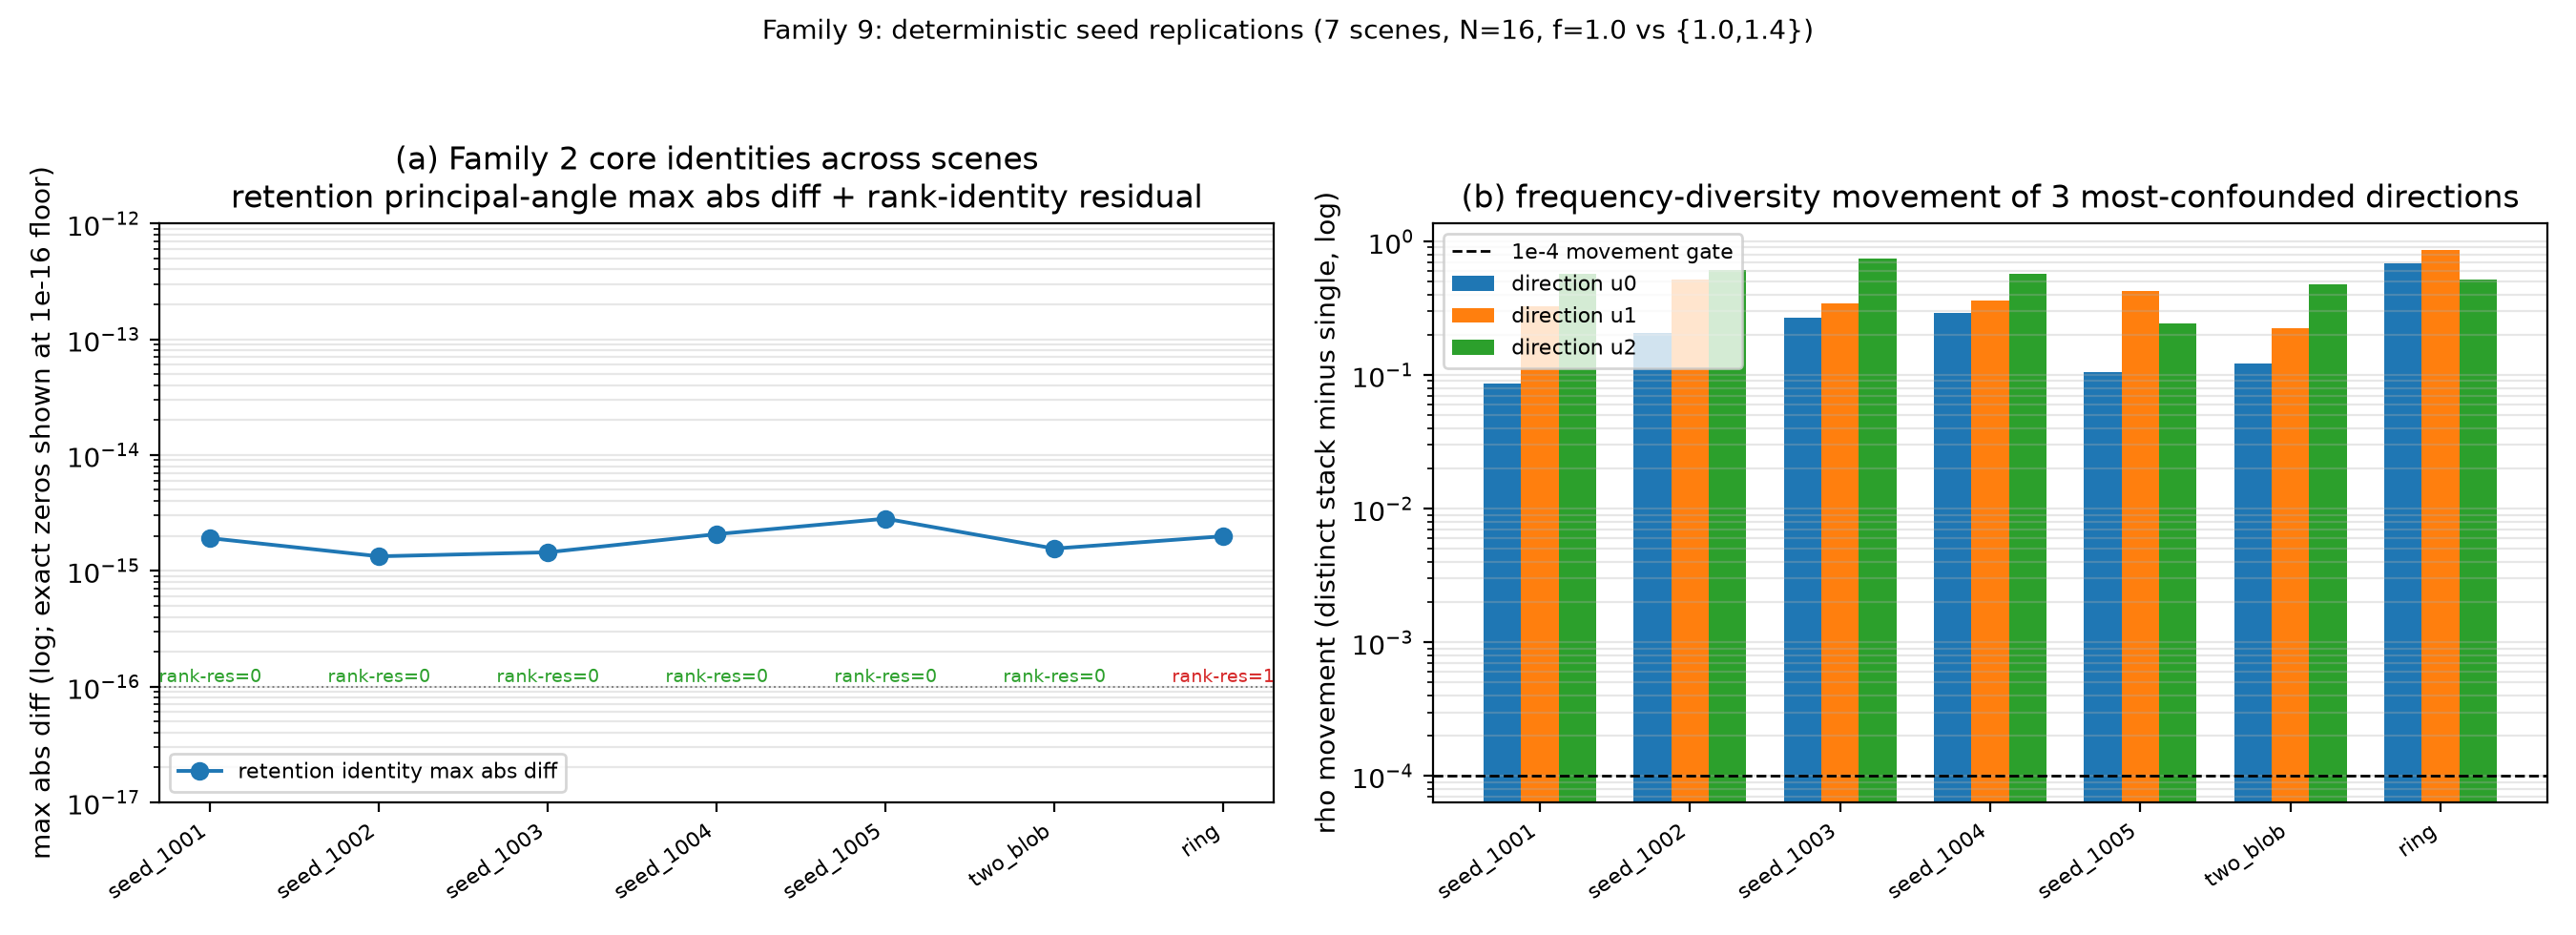
\includegraphics[width=0.86\textwidth]{../figures/family9_seed_replications.png}
\caption{Family 9 seed replications of the algebraic and frequency-diversity
checks.}
\label{fig:f9_seeds}
\end{figure}

\begin{figure}[htbp]
\centering
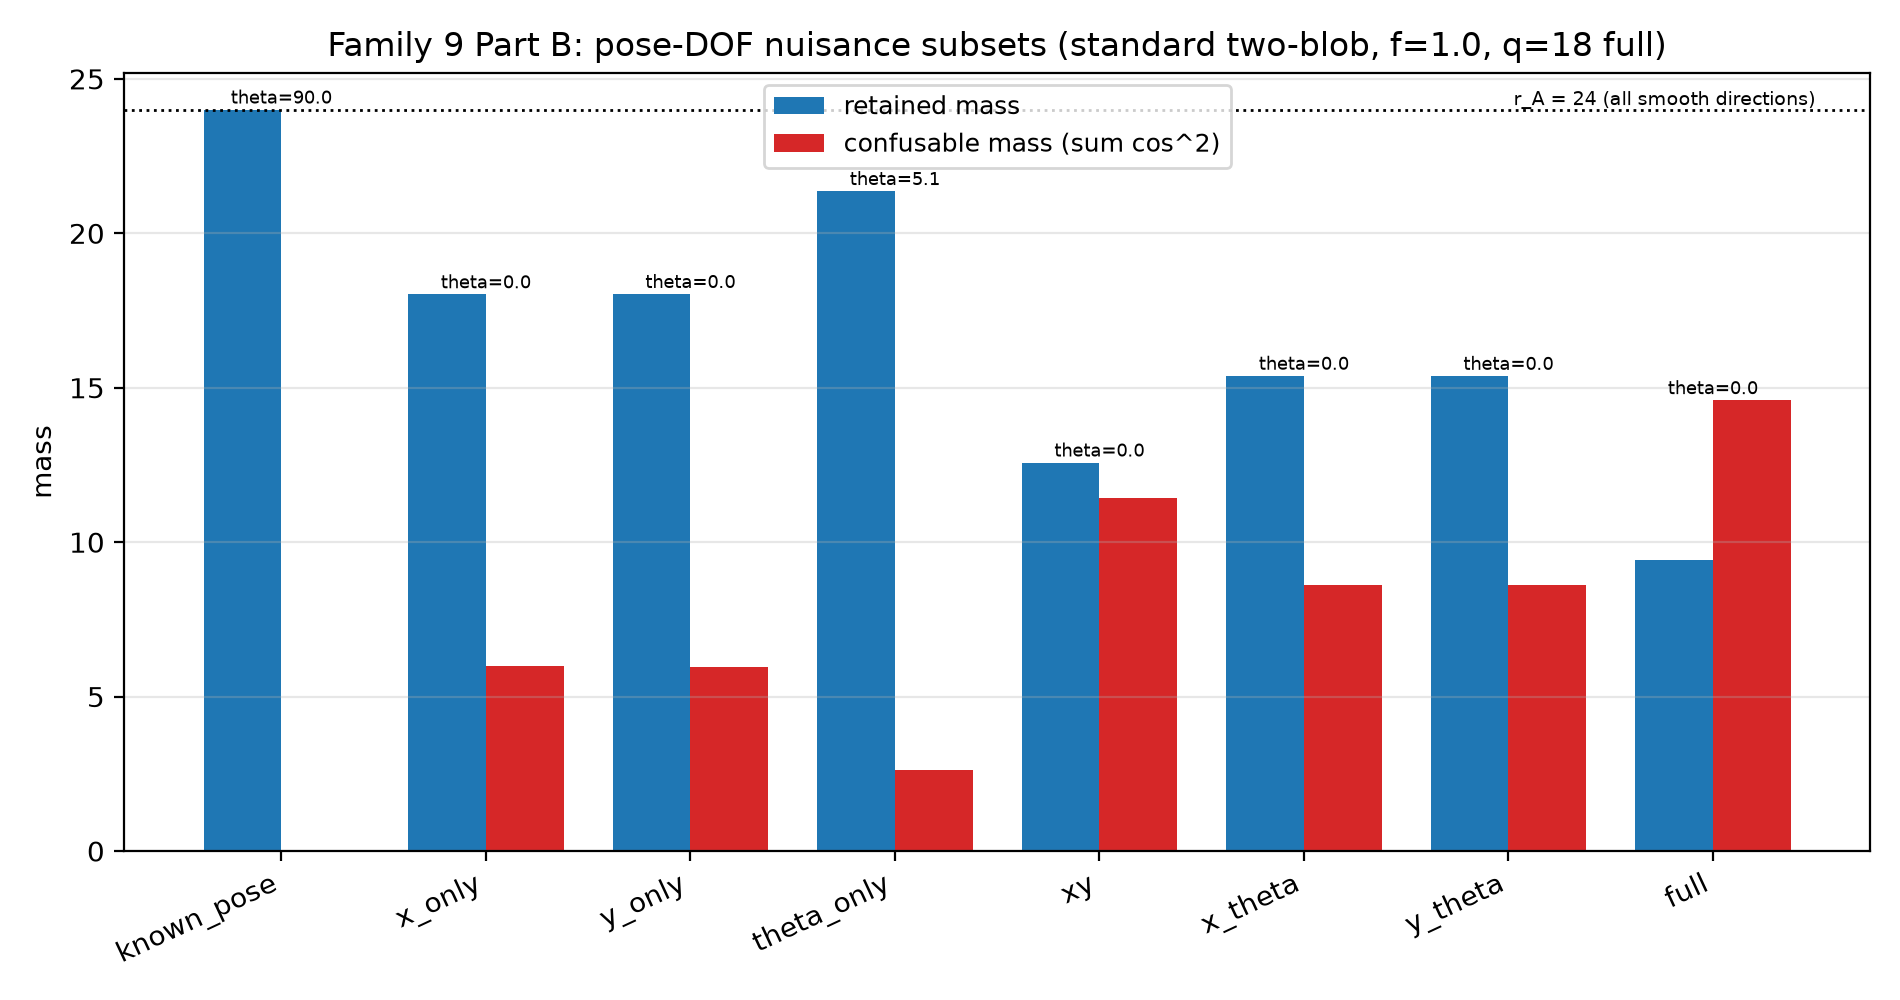
\includegraphics[width=0.86\textwidth]{../figures/family9_pose_dof_ablation.png}
\caption{Family 9 pose-DOF nuisance ablation.}
\label{fig:f9_dof}
\end{figure}

\begin{figure}[htbp]
\centering
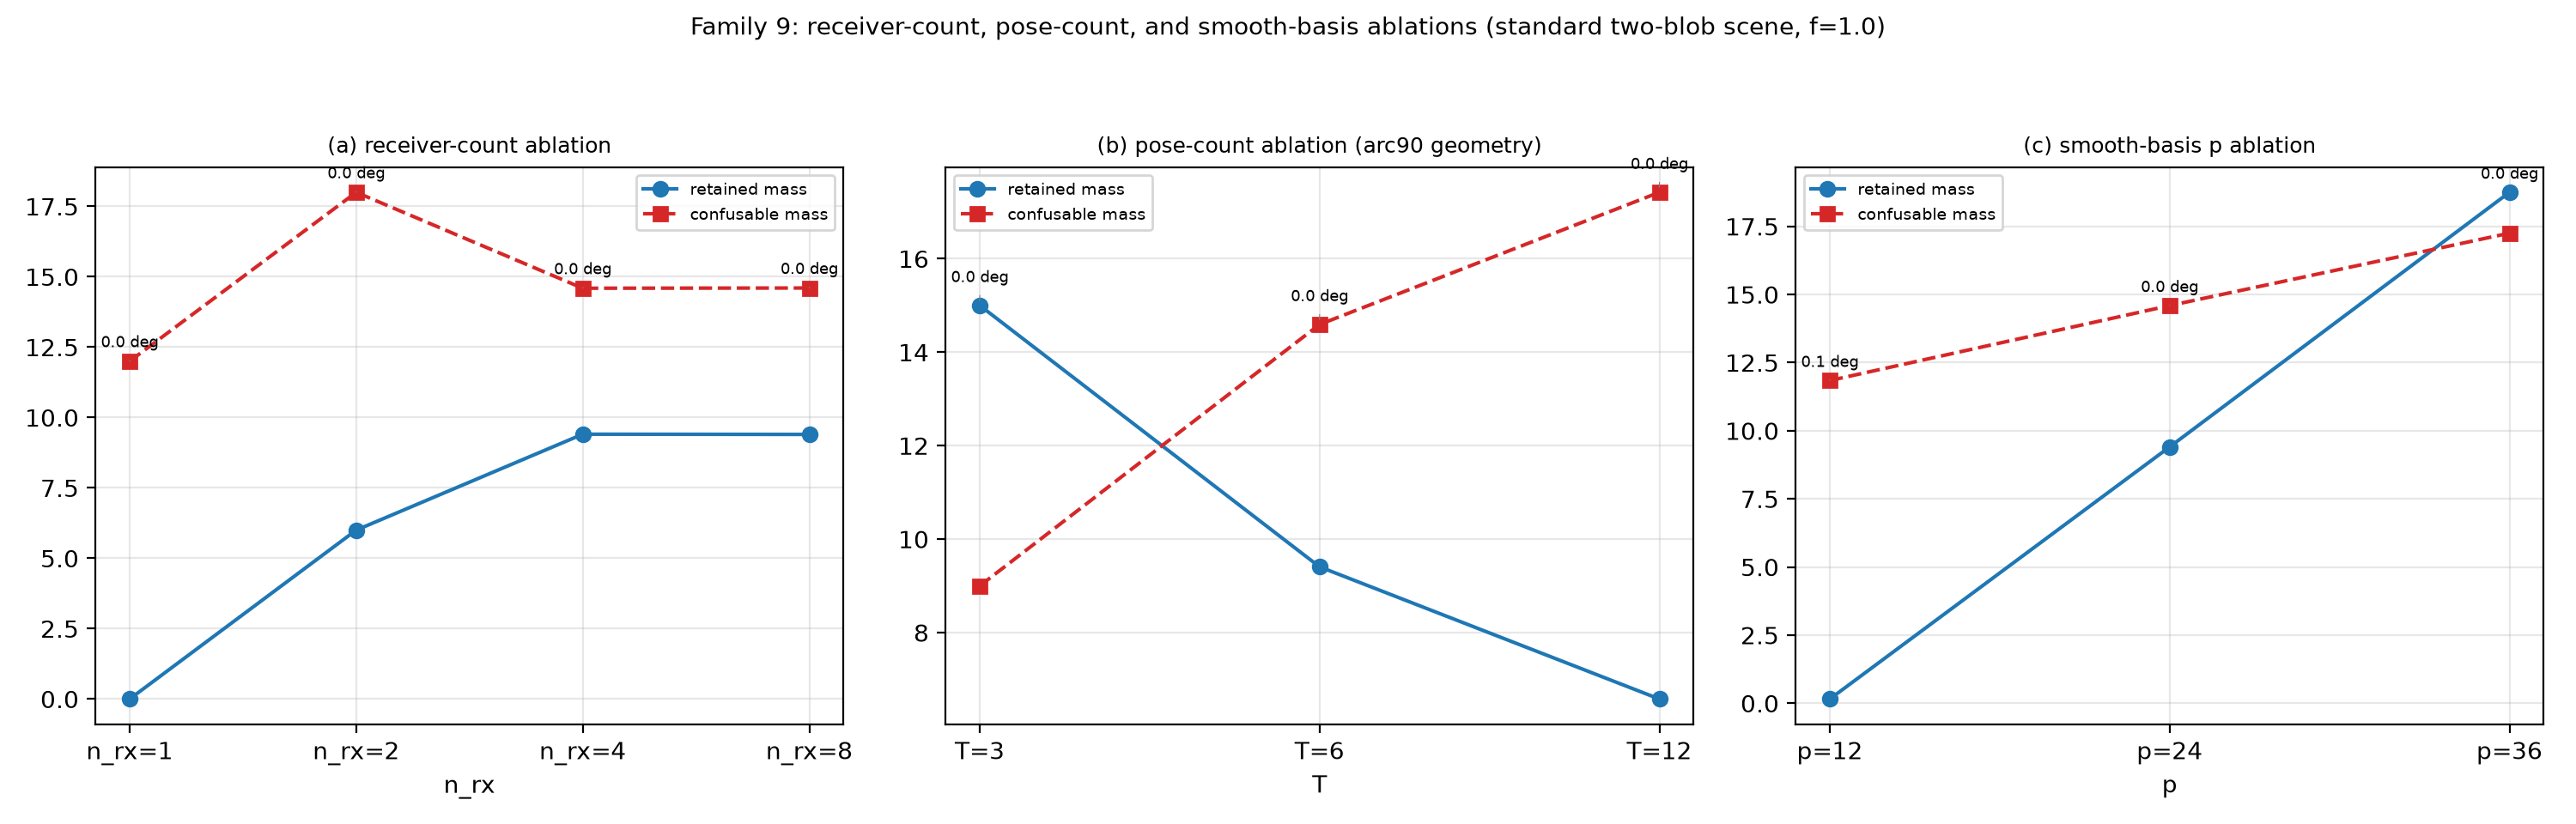
\includegraphics[width=0.86\textwidth]{../figures/family9_rx_T_basis_ablation.png}
\caption{Family 9 receiver-count, pose-count, and basis ablations.}
\label{fig:f9_rx}
\end{figure}

\subsection{Derived operator-Lipschitz bound (Family 5b2)}\label{sec:family5b2}

Family 5b2 corrects the loose structural bound of Family 5b and derives an
alpha-aware tight bound for the affine tangent model. The earlier family
replaced $\|C^{-1}\|_2$ by the general $\alpha\ge0$ bound
$1/\sigma_{\min}(B)^2$, which blew up as $\sigma_{\min}^{-4}$ despite
$\alpha=1.0$; the Family 5b constant $L_{\mathrm{struct}}=1.408\times10^7$ is
cited here only as corrected. Family 5b2 uses the exact
$\|C^{-1}\|_2=1/(\sigma_{\min}(B)^2+\alpha)$ for the PSD-plus-shift
$C=B^TB+\alpha I$ \FDL{}, extends the affine certificate to every
$\epsilon\ge0$ (the $\alpha$ floor keeps $C_{\mathrm{aff}}$ invertible), and
evaluates the actual radius-$\epsilon$ Lipschitz quotient on
$d=\epsilon u$.

\begin{table}[htbp]
\centering
\small
\caption{Family 5b2 tight Lipschitz ingredients and affine certificate
(\texttt{results/family5b2\_alpha\_tight.json}).}
\label{tab:f5b2}
\begin{tabular}{l l}
\toprule
quantity & value \\
\midrule
pointwise $L_{\mathrm{struct,tight}}(X_0)$ &
$1.124\times10^{-2}$ \\
loose Family 5b $L_{\mathrm{struct}}(X_0)$ (corrected) &
$1.408\times10^7$; tightness ratio $1.252285\times10^9$ \\
term balance & A-term $1.097\times10^{-2}$ (97.53\%);
regularised B/P term $2.783\times10^{-4}$ (2.47\%) \\
affine certificate (2000 directions, seed 7171) &
valid for $\epsilon\in\{10^{-3},3\times10^{-3},10^{-2},3\times10^{-2},10^{-1}\}$; \\
 & all fro/lambda checks true; $L_{\mathrm{cert,affine}}$ from
$1.131\times10^{-2}$ to $1.831\times10^{-2}$ \\
full nonlinear samples (500 directions, seed 9191) &
worst Frobenius quotient $3.228\times10^{-4}<L_{\mathrm{struct,tight}}(X_0)$; \\
 & no sampled violations; sampled envelope $1.125\times10^{-2}$ \\
FD Jacobian validation & global rel.\ Fro J$_A$ $5.991\times10^{-7}$,
J$_B$ $5.374\times10^{-7}$; O($h^2$) ratios $\sim4$ \\
\bottomrule
\end{tabular}
\end{table}

The tight pointwise constant is $L_{\mathrm{struct,tight}}(X_0)=1.124\times10^{-2}$,
an improvement by factor $1.252285\times10^9$ over the loose Family 5b value
of $1.408\times10^7$, and the balance reverses: the $A$-term supplies 97.53\%
of the tight constant while the regularised $B/P$ term contributes only
2.47\%. The affine tangent certificate is rigorous for the affine model
conditional on the numerically checked finite-difference Jacobians \FDL{}:
with $\alpha>0$, $C_{\mathrm{aff}}$ remains invertible for every
$\epsilon$ in the tested set up to $0.1$, and none of the 2000-direction
frobenius or eigenvalue-drop checks violates the certificate. The full
nonlinear model has no sampled violations either, but that result is a
derived structural bound with a sampled ingredient envelope, not a formal
nonlinear interval certificate \OBS{}: no uniform radius-$\epsilon$ bounds
on the nonlinear ingredients are proven.

\begin{figure}[htbp]
\centering
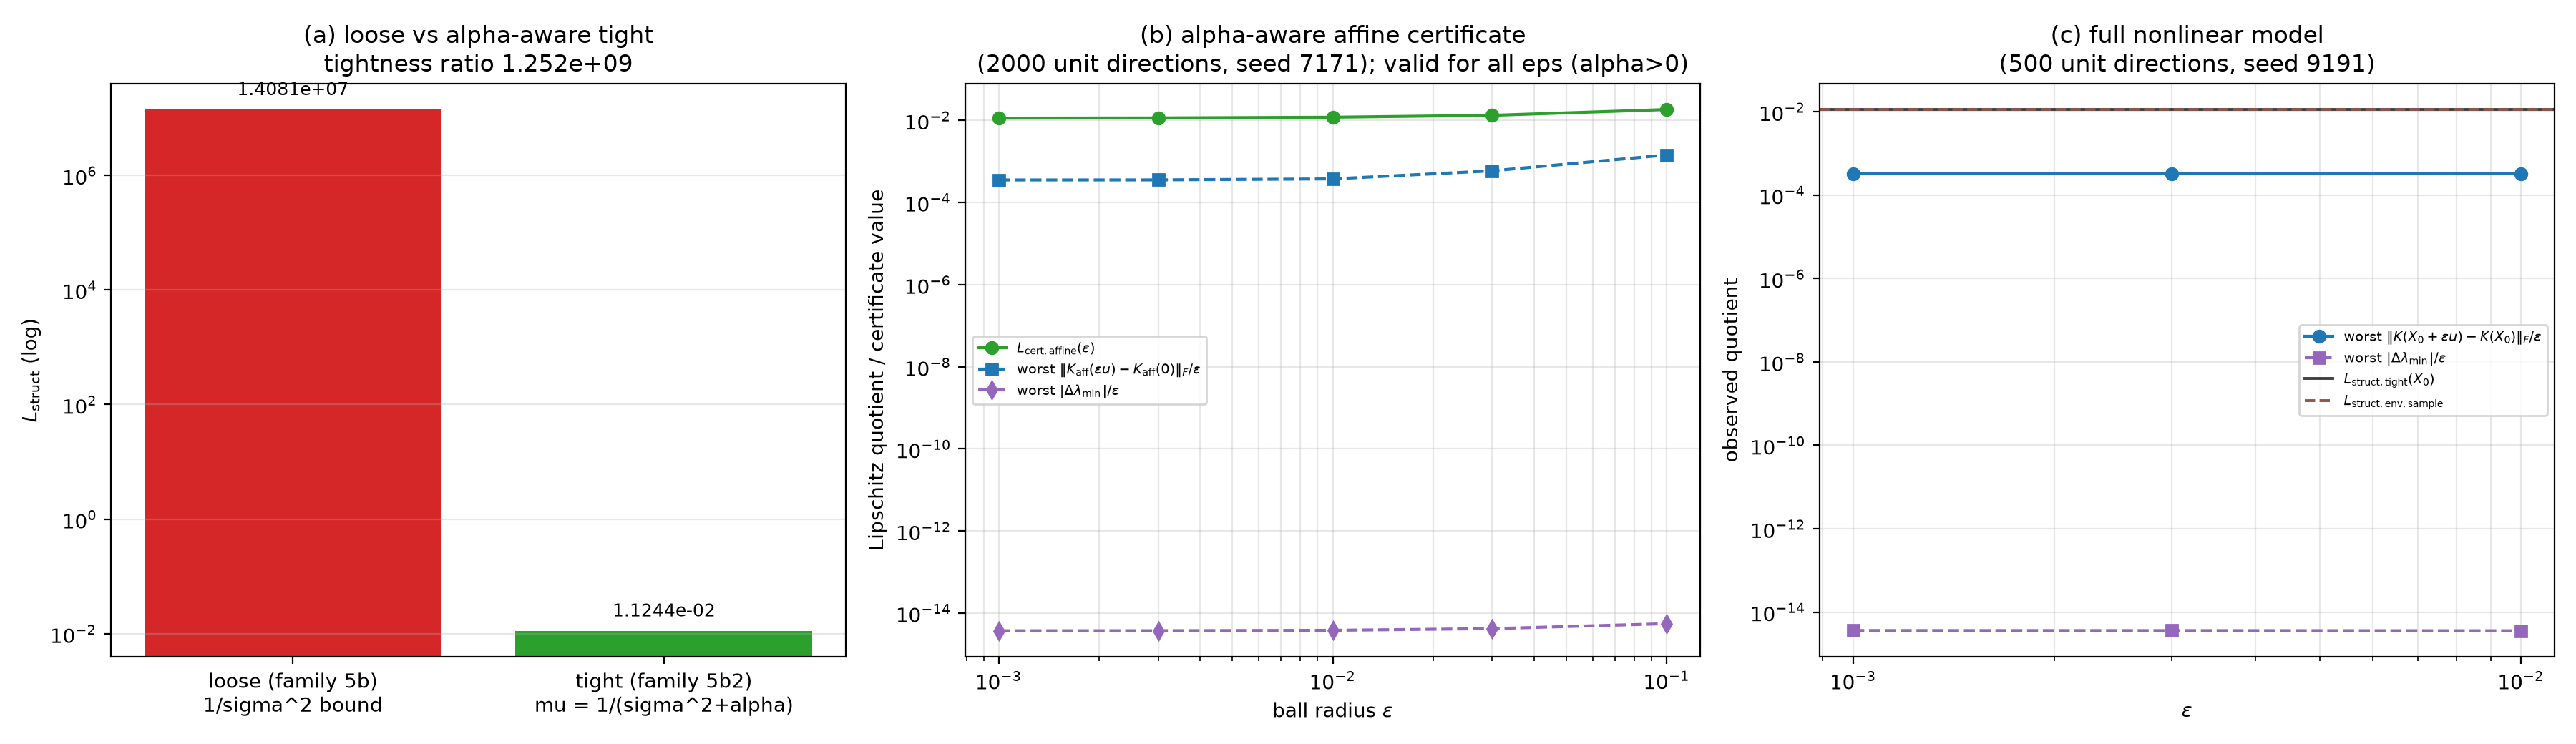
\includegraphics[width=0.86\textwidth]{../figures/family5b2_alpha_tight.png}
\caption{Family 5b2 alpha-aware tight Lipschitz certificate.}
\label{fig:f5b2}
\end{figure}

\section{Related work}\label{sec:related}

The ingredients that this study combines are mature and are not claimed as
novel. Schur-complement and pseudoinverse elimination of nuisance parameters,
including linear least-squares formulations with explicit stability analysis,
appears in the self-calibration and bilinear inverse-problem framework of
Ling and Strohmer~\cite{ling}. In inverse source scattering, Entekhabi and
Isakov~\cite{entekhabi} show increasing stability when many frequencies are
used in two dimensions, providing a continuum-level reason why genuinely
diverse frequencies can reduce ambiguity in source-type problems. For
volumetric microwave imaging, Shea et al.\ \cite{shea} validate a
multiple-frequency inverse-scattering technique on realistic numerical breast
phantoms, establishing multi-frequency volumetric inversion as an operating
regime this study does not re-derive. Weidling and Hohage~\cite{weidling}
verify variational source conditions and stability estimates for inverse
electromagnetic medium scattering, which frame how stability statements are
to be obtained in the infinite-dimensional setting. On the SLAM side,
4D-radar SLAM literature treats pose/map estimation and loop closure with
all-weather sensing: Burnett et al.\ \cite{burnett} compare radar-only and
lidar-only mapping/localization in practice, and Hilger et al.\ \cite{hilger}
investigate introspective loop closure for 4D radar SLAM. These works make
radar SLAM an engineering context in which the checked pose-confounding
operators would have to operate; they do not themselves analyze the
principal-angle retention law studied here.

The synthesis boundary is therefore precise: Schur-complement nuisance
elimination, principal angles, gauge analysis, multi-frequency stability, and
radar SLAM are all established ingredients. The tested contribution of this
draft is the explicit finite-dimensional pose-confounding retention theory for
whitened/realified full-wave contrast-source SLAM tangents, together with its
executable numerical consequences and preserved counterexamples. This draft
contains no ``first'' and no ``no prior work'' claim, and the novelty boundary
is retrieval-bounded.

\section{Limitations and open questions}\label{sec:limits}

All executed claims are finite-dimensional. The following therefore remain
open:
\begin{itemize}
\item \emph{Continuum transfer and stable transversality.} The finite
discrete identities do not prove closed-range properties,
$\inf_{Au\ne0}\mathrm{dist}(Au,\mathrm{Range}(B))/\|Au\|>0$, or convergence of
the retention spectrum under discretization. Family 7 refinement is a
finite-grid diagnostic only: the decreasing $\theta_{\min}$ trend and the
constant near-confounded count are observed on N=16..48, with no continuum
convergence or stable-transversality theorem. \OPN{}
\item \emph{Rank events and transversality.} No rank event occurred along the
Family 5 random path or the Family 7 frequency sweep; the 21 literal
near-crossing flags sit in the lowest numerical near-null pairs of
$K_{\mathrm{eff}}$ and are not certified crossings. Continuity/rank-event
theory for the retention spectrum near gap closure remains open, and only
cluster/projector treatments are admissible there. \OPN{}
\item \emph{Global nonlinearity and cycle skipping.} The local tangent/Fisher
formulation does not address cycle skipping, phase wrapping, wrong data
association, posterior multimodality, or basins of attraction. \OPN{}
\item \emph{Colored-noise realism.} Family 6 declares a synthetic covariance
$C_f=\sigma_f^2(I_T\otimes R_{\mathrm{rx}})$ with a Mat\'ern-1/2 receiver
factor and per-frequency SNR normalization; the whitening and algebraic
checks pass under that declared model only. Physical realism, measured noise
covariance, and estimator-level correlated-noise behaviour are not
established. \OPN{}
\item \emph{Trajectory normalization and standoff.} Family 4c per-pose
$A$-block normalization is a declared gain control, not a physical noise
covariance or an optimal-SNR whitening rule. Same standoff fixes curved-path
range but changes design/polyline length with angular coverage, and the
straight path still varies standoff, so no universal trajectory-ordering
theorem is asserted. \OPN{}
\item \emph{SOM/current-space distinction.} Family 8 checks, on the tested
finite scenario, that the current-space $G_S$ composition and range
containment hold while the $V_{GS}$/SOM and map-tangent $V_A$/$K_{\mathrm{eff}}$
mode subspaces are distinct. This is numerical evidence, not a continuum
theorem, and no pullback/composition theorem $A=G_ST_\chi$ or SOM quality
claim was proved. \OPN{}
\item \emph{Interval Lipschitz certification.} Formal interval certification of
the full nonlinear operator-Lipschitz constant remains open. The Family 5b2
affine tangent certificate is rigorous for the affine model only and remains
conditional on the numerically computed finite-difference Jacobians; the
full-model result is a derived structural bound with a sampled ingredient
envelope, not a formal interval certificate. \OPN{}
\item \emph{Gauge converses.} Zero retention in a tested direction does not
imply that direction is a physical group gauge, and the p=24 smooth-basis
representation limits the gauge conclusions of Family 3. Exact global SE(2)
equivariance is not available on the bounded boxed grid. \OPN{}
\end{itemize}

\section{Reproducibility}\label{sec:repro}

All runs were executed from this experiment root on Apple Silicon CPU
(macOS-26.6.2 arm64; Python 3.12.13; numpy 2.5.2; scipy 1.18.1; matplotlib
3.11.1). The exact recorded commands are:
\begin{verbatim}
.venv/bin/python -m unittest discover -s src -p "test_*.py" -v
.venv/bin/python src/validate_self_cell.py
.venv/bin/python src/family1_pilot.py
.venv/bin/python src/family1_grid_refinement.py
.venv/bin/python src/family2_algebraic_spine.py
.venv/bin/python src/family2_parent_correction.py
.venv/bin/python src/family3_gauge_born.py
.venv/bin/python src/family3_parent_correction.py
.venv/bin/python src/family3b_refinements.py
.venv/bin/python src/family4_frequency_trajectory.py
.venv/bin/python src/family4b_normalized_control.py
.venv/bin/python src/family4_parent_controls.py
.venv/bin/python src/family5_sensitivity.py
.venv/bin/python src/family4c_trajectory_control.py
.venv/bin/python src/family6_colored_noise.py
.venv/bin/python src/family7_refinement_rank.py
.venv/bin/python src/family8_som_distinction.py
.venv/bin/python src/family9_replications_ablation.py
.venv/bin/python src/family5b_lipschitz_bound.py
.venv/bin/python src/family5b2_alpha_tight.py
\end{verbatim}
Recorded wall runtimes: unit tests 5.43 s; self-cell validation 5.12 s;
grid refinement 5.76 s total; Family 1 pilot 2.14 s; Family 2 4.25 s; Family 3
4.81 s; Family 3b 5.54 s; Family 4 0.78 s; Family 4b 0.17 s; Family 5 18.04 s.
Round-2 wall runtimes: Family 4c 0.147 s; Family 6 1.15 s; Family 7 18.54 s;
Family 8 0.45 s; Family 9 1.35 s; Family 5b 40.87 s (read-only precursor,
corrected by Family 5b2); Family 5b2 41.19 s.
Deterministic seeds are listed in each JSON (map seeds 0/1/2; pose seeds
10/11/12; unit-test seeds 12345/54321/2026; gauge Born seed 31415; Family 5
seeds 2718/9191; round-2 Monte-Carlo whitening seeds 2718/4242/5150; Family 9
scene seeds 1001--1005 plus the two-blob and ring scenes; Family 5b/5b2
direction seeds 7171/9191/5353). Raw machine-readable outputs, figures, source SHA-256
digests, and per-family ``cannot establish'' sections are stored as follows
(see \texttt{notes/synthesis.md} and \texttt{notes/manuscript\_sources.md} for the full
mapping):
\begin{itemize}
\item results: \texttt{results/family1\_pilot\_results.json},
\texttt{results/family1\_grid\_refinement.json},
\texttt{results/self\_cell\_quadrature\_validation.json},
\texttt{results/family2\_results.json}, \texttt{results/family2\_parent\_correction.json},
\texttt{results/family3\_gauge\_born.json}, \texttt{results/family3\_parent\_correction.json},
\texttt{results/family3b\_refinements.json}, \texttt{results/family4\_results.json},
\texttt{results/family4b\_normalized\_control.json},
\texttt{results/family4\_parent\_controls.json}, \texttt{results/family5\_sensitivity.json},
\texttt{results/family4c\_trajectory\_control.json},
\texttt{results/family6\_colored\_noise.json},
\texttt{results/family7\_refinement\_rank.json},
\texttt{results/family8\_som\_distinction.json},
\texttt{results/family9\_replications\_ablation.json},
\texttt{results/family5b\_lipschitz\_bound.json},
\texttt{results/family5b2\_alpha\_tight.json}.
\item notes: the family reports and parent-correction notes listed in
\texttt{notes/manuscript\_sources.md}; round-2 reports are
\texttt{notes/family6\_report.md}, \texttt{notes/family4c\_trajectory\_control.md},
\texttt{notes/family7\_refinement\_rank.md}, \texttt{notes/family8\_som\_distinction.md},
\texttt{notes/family9\_replications\_ablation.md},
\texttt{notes/family5b\_lipschitz\_bound.md} (corrected precursor), and
\texttt{notes/family5b2\_alpha\_tight.md}; the consolidated read-only round-2
synthesis is \texttt{notes/synthesis\_round2.md}.
\item figures: \texttt{figures/family1\_fd\_convergence.png},
\texttt{figures/family1\_grid\_refinement.png},
\texttt{figures/family2\_retention\_spectra.png},
\texttt{figures/family2\_prior\_sweep.png}, \texttt{figures/family2\_duplicate\_prior\_effect.png},
\texttt{figures/family3\_gauge\_residuals.png}, \texttt{figures/family3\_gauge\_refinement.png},
\texttt{figures/family3\_anchor\_rho.png}, \texttt{figures/family3\_born\_empty\_background.png},
\texttt{figures/family3b\_gauge\_pixel\_refinement.png},
\texttt{figures/family3b\_anchor\_generator\_retention.png},
\texttt{figures/family3b\_born\_bilinear\_refined.png},
\texttt{figures/family4\_monotonicity.png}, \texttt{figures/family4\_duplicate.png},
\texttt{figures/family4\_shared\_z.png}, \texttt{figures/family4\_trajectories.png},
\texttt{figures/family4b\_normalized\_shared\_z.png},
\texttt{figures/family5\_derivative\_formula.png},
\texttt{figures/family5\_eigenvalue\_prediction.png},
\texttt{figures/family5\_robust\_surrogate.png}, \texttt{figures/family5\_rank\_events.png},
\texttt{figures/family4c\_trajectory\_control.png},
\texttt{figures/family6\_snr\_sweep.png}, \texttt{figures/family6\_correlation\_effect.png},
\texttt{figures/family6\_noise\_whitening\_sanity.png},
\texttt{figures/family6\_retention\_spectra\_colored.png},
\texttt{figures/family7\_resolution\_convergence.png},
\texttt{figures/family7\_frequency\_rank\_sweep.png}, \texttt{figures/family7\_contrast\_sweep.png},
\texttt{figures/family8\_composition\_identity.png}, \texttt{figures/family8\_mode\_distinction.png},
\texttt{figures/family9\_seed\_replications.png}, \texttt{figures/family9\_pose\_dof\_ablation.png},
\texttt{figures/family9\_rx\_T\_basis\_ablation.png},
\texttt{figures/family5b\_lipschitz\_bound.png}, \texttt{figures/family5b2\_alpha\_tight.png}.
\item invalidated pre-correction snapshot (preserved verbatim):
\texttt{archive/INVALIDATED\_self\_cell\_2026-09-03T092339Z/}.
\end{itemize}
Round-2 families were executed with \texttt{.venv/bin/python} from this
experiment root. Each new round-2 result JSON embeds the exact command,
generated-UTC timestamp, configuration, and script/reused-module SHA-256
digests; \texttt{results/family5b\_lipschitz\_bound.json} is retained read-only
as the corrected precursor.
Source SHA-256 digests are embedded in each result JSON and repeated in the
notes; checksums for the archive are in the archive \texttt{checksums.txt}.

\section{AI-use and integrity disclosure}\label{sec:ai}

AI tools were used in this workflow as required by the workflow license,
including drafting of this manuscript, and the experiment itself was produced
by an AI-assisted agentic workflow operating in this working directory. All
numerical claims in this manuscript were machine-verified against the raw JSON
result files in this working directory during manuscript production; no
experiment was rerun for this write-up, and no number was fabricated or
relabelled. Round-2 families were executed with \texttt{.venv/bin/python},
and their source/config SHA-256 digests and recorded configurations are
embedded in the new result JSON files listed in
Section~\ref{sec:repro}. Every recorded failure and counterexample cited here remains
visible in the JSON records and the per-family reports. The claims are scoped
as finite-dimensional numerical evidence on a deterministic synthetic harness,
not as production, physical, online-SLAM, continuum, or novelty acceptance.
No external data, secrets, or protected reasoning content were used or
persisted.

\appendix
\section{Claim-status tables}\label{app:claims}

The following tables repeat, family by family, the recorded claim statuses
(PASS / FAIL / NOT MET / flagged / observed / recorded). They match
\texttt{notes/synthesis.md} sections 1.1--1.6; the round-2 tables match the
consolidated claim table in \texttt{notes/synthesis\_round2.md}.

\subsection{Family 1}
\begin{table}[ht]
\centering
\small
\caption{Family 1 claim statuses (as executed).}
\label{app:tab:f1}
\begin{tabular}{p{0.42\textwidth} p{0.16\textwidth} p{0.38\textwidth}}
\toprule
claim & status & key evidence \\
\midrule
corrected self-cell v2 matches direct quadrature & PASS (finite ladder) &
max abs quadrature error $3.13\times10^{-16}$ \\
$\nabla_s g=-\nabla_z g$ preserved & PASS &
corrected rel err $1.7\times10^{-9}$ vs 2.0 old sign \\
map-Jacobian FD consistency O(h$^2$) & PASS &
rel err at h=$10^{-3}$ $2.25\times10^{-9}$..$1.74\times10^{-8}$; slope 1.98 \\
pose-Jacobian FD consistency O(h$^2$) & PASS &
rel err $8.38\times10^{-7}$..$4.09\times10^{-6}$; slope 2.0000 \\
non-resonant state margin & PASS &
$\sigma_{\min}(M)/\|M\|=0.7189$; residual $9.3\times10^{-16}$ \\
Born/full-wave trend & PASS (recorded) &
rel F $1.8\times10^{-3}$..$3.5\times10^{-2}$ for s=0.01..0.2 \\
grid refinement N16/24/32/40 & PASS (diagnostic) &
rel diff vs N=40 $1.45\times10^{-3}$..$1.60\times10^{-4}$ \\
\bottomrule
\end{tabular}
\end{table}

\subsection{Family 2}
\begin{table}[ht]
\centering
\small
\caption{Family 2 claim statuses (as executed). Pixel/smooth unless noted.}
\label{app:tab:f2}
\begin{tabular}{p{0.40\textwidth} p{0.18\textwidth} p{0.38\textwidth}}
\toprule
claim & status & key evidence \\
\midrule
$\ker K_{\mathrm{SLAM}}=\{u: Au\in\mathrm{Range}(B)\}$ &
PASS (smooth); pixel gate FAIL, identity certified &
dist 0 (smooth); pixel dist $8.47\times10^{-7}$ vs $10^{-8}$; nullity 226=226 \\
rank identity & PASS & residual 0 both bases \\
retention = 1$-\sigma_i^2$, padded & PASS &
residuals $2.89\times10^{-15}$/$1.55\times10^{-15}$ \\
$\le r_B$ values differ from 1 & PASS & count 18=18=$r_B$ \\
$\mathrm{rank}\,L_X\le\mathrm{rank}\,B$ & PASS & max factor rank 18=$r_B$ \\
PSD order and interlacing & PASS &
violations $5.0\times10^{-21}$/$6.7\times10^{-21}$ \\
$\alpha\to0$ limit & PASS (limiting) &
d0($10^{-14}$)=$5.70\times10^{-9}$/$3.67\times10^{-9}$ \\
$\alpha\to\infty$ regular limit & PASS &
dinf($10^4$)=$5.17\times10^{-7}$/$5.50\times10^{-7}$ \\
finite-prior shrinkage & PASS &
$\rho_X\in(0.086,1]$ at $\alpha=10^{-3}$ \\
singular-prior non-convergence & PASS (magnitude example not met) &
$\mathrm{dinf}_s(10^4)$=$4.71\times10^{-4}$/$2.30\times10^{-4}$ \\
duplicate no-prior / fixed prior / joint prior &
PASS / observed / PASS &
max rho diff $6.7\times10^{-16}$ / $3.99\times10^{-2}$ / $1.7\times10^{-15}$ \\
stable $C^TC$ factorization & PASS &
residual $3.77\times10^{-16}$/$2.70\times10^{-16}$ \\
smooth c1-c3 at N=32/40 & PASS &
c1 dist 0; c3 residuals $1.90\times10^{-15}$/$8.24\times10^{-15}$ \\
\bottomrule
\end{tabular}
\end{table}

\subsection{Family 3 and 3b}
\begin{table}[ht]
\centering
\small
\caption{Family 3 (raw) and Family 3b (corrected-condition) claim statuses.}
\label{app:tab:f3}
\begin{tabular}{p{0.42\textwidth} p{0.18\textwidth} p{0.36\textwidth}}
\toprule
claim & status & key evidence \\
\midrule
smooth SE(2) gauge residual $\le5\times10^{-2}$, decreasing & FAIL &
Tx $0.183\to0.183$, Ty 0.0865, Rot $0.310\to0.309$; \\
 & & representation residuals 0.78/0.57/0.70 \\
smooth generator in ker $K_{\mathrm{SLAM}}$ & NOT MET at gauge level &
kernel distances $10^{-8}$..$10^{-9}$ \\
pixel-basis larger-residual control & expected direction NOT reproduced &
residuals $6.6\times10^{-5}$/$1.6\times10^{-5}$/$4.7\times10^{-5}$ \\
symmetric rotation not a map gauge & PASS (pose-only stabilizer) &
$\|\delta\chi_{\mathrm{rot}}\|=7.8\times10^{-17}$; \\
 & & $\|B\,\delta X_{\mathrm{rot}}\|=1.9\times10^{-6}$ \\
anchors raise global $\rho_{\min}$ $>$10x & FAIL &
ratios 1.26 / 0.011 / 0.244 \\
$B=0$ and $K_{\mathrm{SLAM},0}=K_{\mathrm{IS},0}$ at empty background &
PASS & 0.0 / 0.0 (relative Frobenius) \\
bilinear term dominates linear term & PASS (metric) & ratio 2.81 \\
full-wave FD matches bilinear term (O(h$^2$), $<10^{-3}$) & FAIL &
rel err 0.218, h-independent \\
remainder R(h)-R0 slope two & NOT MET & slope 1.015 \\
3b pixel residual $\le10^{-3}$, non-increasing & FAIL (magnitude PASS) &
Tx $6.61\to7.95\to8.14\times10^{-5}$ \\
3b pixel kernel distance tiny/decreasing & PASS &
Tx $3.96\to1.22\to0.81\times10^{-10}$ \\
3b augmented p27 representation/gauge & PASS &
rep residuals $10^{-15}$; gauge equals pixel floor \\
3b generator-specific anchor & PASS &
base $\rho_g$ $9.91\times10^{-11}$; \\
 & & corner ratio 11.93; disk 2.19e5; ring 166 \\
3b $A(0)$ equals Born map & PASS & rel Frobenius $7.05\times10^{-17}$ \\
3b Born FD slope gate & FAIL / not established (degenerate) &
value $2.3\times10^{-13}<10^{-4}$, slope $-1.0$ \\
3b full-wave chi$^2$ floor / remainder drift & PASS &
floor $2.166\times10^{-4}$; drift slope 1.986 \\
\bottomrule
\end{tabular}
\end{table}

\subsection{Family 4, 4b, and parent controls}
\begin{table}[ht]
\centering
\small
\caption{Family 4 claim statuses (raw, normalized control, parent controls).}
\label{app:tab:f4}
\begin{tabular}{p{0.42\textwidth} p{0.18\textwidth} p{0.36\textwidth}}
\toprule
claim & status & key evidence \\
\midrule
PSD monotonicity under distinct stacking & PASS &
min eig increments $1.29\times10^{-14}$..$1.52\times10^{-13}$ \\
duplicate no-prior invariance & PASS & max |rho| $1.19\times10^{-12}$ \\
fixed finite prior changes rho & observed (expected) &
max |rho| change 0.0398 at $\alpha=1$ \\
jointly scaled prior invariance & PASS & max |rho| $1.22\times10^{-15}$ \\
distinct frequency separates confounded directions & PASS &
3/3 above $10^{-4}$ \\
duplicate leaves rho fixed & PASS & max movement $2.9\times10^{-16}$ \\
trajectory hypothesis (retained mass order) & FAIL (counterexample) &
observed arc90 $>$ straight $>$ circle360 $>$ arc180 \\
trajectory confusable-mass order & FAIL (counterexample) &
observed arc180 $>$ circle360 $>$ straight $>$ arc90 \\
block-normalized control (4b) & PASS &
movements 0.106/0.194/0.382; \\
 & & duplicate $<10^{-10}$; monotonicity 4/4 \\
SNR-matched frequency diversity (parent) & PASS &
retentions 0.117/0.216/0.446 \\
trajectory metric/standoff sensitivity (parent) & observed &
same-radius order arc90 $>$ arc180 $>$ circle360 \\
\bottomrule
\end{tabular}
\end{table}

\subsection{Family 5}
\begin{table}[ht]
\centering
\small
\caption{Family 5 claim statuses (as executed).}
\label{app:tab:f5}
\begin{tabular}{p{0.42\textwidth} p{0.18\textwidth} p{0.36\textwidth}}
\toprule
claim & status & key evidence \\
\midrule
P1 full derivative vs FD & PASS & rel err $6.25\times10^{-7}$; slope 1.91 \\
P1 frozen-nuisance clearly worse & PASS & rel err $4.44\times10^{-2}$ \\
P2 first-order gapped eigenvalues & PASS &
errors $8.0\times10^{-8}$/ $1.1\times10^{-7}$; slopes $\sim2$ \\
P2 frozen $>$10x full on gapped & PASS & ratios 39.4x / 14.8x \\
P2 median gap condition & flagged (excluded) &
gap $5.94\times10^{-8}<10^{-6}$, idx 12 \\
P3 robust surrogate & PASS &
err($10^{-2}$) $4.46\times10^{-5}$; slope 2.00 \\
P4 Weyl self-check & PASS (empirical only) &
violations 0; no certified constant \\
P5 rank/event scan & observed (no forced pass) &
min gap $6.62\times10^{-15}$; no rank event \\
\bottomrule
\end{tabular}
\end{table}

\subsection{Family 6}
\begin{table}[ht]
\centering
\small
\caption{Family 6 claim statuses (as executed).}
\label{app:tab:f6}
\begin{tabular}{p{0.42\textwidth} p{0.18\textwidth} p{0.36\textwidth}}
\toprule
claim & status & key evidence \\
\midrule
analytic whitening $W_fC_fW_f^H=I$ & PASS &
rel.\ Fro $7.370\times10^{-16}$/$5.550\times10^{-16}$/$5.769\times10^{-16}$ \\
Monte-Carlo whitening & recorded &
seed-2718 rel.\ Fro $\sim0.107$ (statistical, not machine whiteness) \\
colored kernel/rank identity & PASS &
residual 0; $r_A$=24, $r_B$=18, $r_{AB}$=42 \\
colored no-prior retention identity & PASS &
max diff $1.776\times10^{-15}$; count $\rho<1$=18 \\
PSD prefix increments at snr$_2$=100 & PASS &
$K_{\mathrm{SLAM}}$ $1.220\times10^{-7}$; $K_{\mathrm{eff}}$ $7.424\times10^{-8}$ \\
duplicate no-prior invariance / fixed prior & PASS / observed &
max $|\Delta\rho|$ $6.216\times10^{-13}$ / $0.3398$ \\
low-SNR drift and finite high-SNR plateau & PASS (tested grid) &
movements $5.8\times10^{-5}$..$5.7\times10^{-1}$; \\
 & & positive tail $0.010$/$0.009$/$0.027$ at $10^{10}$ \\
SNR sweep non-monotonicity & observed & peak at snr$_2$=100
($0.128$/$0.235$/$0.569$), then decline \\
receiver-correlation sweep & recorded (no forced pass) &
$\ell=0.001$..0.5; identity distances are mixed-scale \\
\bottomrule
\end{tabular}
\end{table}

\subsection{Family 4c}
\begin{table}[ht]
\centering
\small
\caption{Family 4c claim statuses (as executed).}
\label{app:tab:f4c}
\begin{tabular}{p{0.42\textwidth} p{0.18\textwidth} p{0.36\textwidth}}
\toprule
claim & status & key evidence \\
\midrule
per-pose $A$-block normalization & PASS &
max $|1-\|A_{\mathrm{block}}\|_F|=2.220\times10^{-16}\le10^{-12}$ \\
raw vs normalized ordering flip & no flip (observed) &
same retained/confusable orders in both columns \\
four-core retained-mass hypothesis & FAIL (counterexample) &
arc90 $>$ straight $>$ arc180 $>$ circle360 \\
four-core confusable-mass hypothesis & FAIL (counterexample) &
arc90 $<$ straight $<$ arc180 $<$ circle360 \\
arc270 lowest retained & observed & 7.5353 (normalized),
below circle360 7.7012 \\
per-pose normalization is a gain control & recorded &
not a physical noise covariance or optimal-SNR rule \\
Family 4 trajectory counterexample & preserved \CTX{} &
arc90 $>$ straight $>$ circle360 $>$ arc180 (raw equal-length set) \\
\bottomrule
\end{tabular}
\end{table}

\subsection{Family 7}
\begin{table}[ht]
\centering
\small
\caption{Family 7 claim statuses (as executed).}
\label{app:tab:f7}
\begin{tabular}{p{0.42\textwidth} p{0.18\textwidth} p{0.36\textwidth}}
\toprule
claim & status & key evidence \\
\midrule
constant ranks over N=16..48 & PASS (computed rows) &
$r_A$=24, $r_B$=18, $r_{AB}$=42; rank identity true at every N \\
$\theta_{\min}$ decreasing trend & observed &
$4.253070\times10^{-4}\to4.188332\times10^{-4}$ deg \\
near-confounded direction count & observed &
[4,4,4,4,4] constant over tested grid \\
frequency rank events & observed/flagged & 0 events over 21 f points \\
frequency near crossings & flagged (literal criterion) &
21 flags; lowest ascending numerical near-null pairs only \\
$s=0$ Born gates & PASS & B/A ratio 0.0; rel.\ Fro 0.0
(both $<10^{-12}$) \\
Born/full discrepancy growth & observed &
$1.894\times10^{-3}$ ($s=0.01$) to $0.1975$ ($s=1$) \\
contrast machine-rank transition & observed (expected) &
$s=0\to0.01$: $r_B$ 0$\to$18; $r_{AB}$ 24$\to$42 \\
finite-grid scope & recorded & diagnostics only; no continuum proof \\
\bottomrule
\end{tabular}
\end{table}

\subsection{Family 8}
\begin{table}[ht]
\centering
\small
\caption{Family 8 claim statuses (as executed).}
\label{app:tab:f8}
\begin{tabular}{p{0.42\textwidth} p{0.18\textwidth} p{0.36\textwidth}}
\toprule
claim & status & key evidence \\
\midrule
full-wave composition identity & PASS &
stack rel.\ Fro 0 (identical float path) \\
Born composition identity & PASS &
rel.\ Fro $7.05442\times10^{-17}$ \\
Range$(A_c)\subseteq$Range$(G_S)$ & PASS &
proj diff $3.5260\times10^{-15}$; residual $2.3354\times10^{-15}$; \\
 & & literal arccos rad gate false (roundoff floor) \\
$V_{GS}$ vs $V_A$ right subspaces distinct & observed &
0/24 angles $<10^{-8}$ deg; median $29.70670$ deg; max $89.79380$ deg \\
$K_{\mathrm{eff}}$ confounded-vector overlaps & recorded &
max squared overlaps $3.2680\times10^{-3}$ ($V_{GS}$) vs \\
 & & $5.7556\times10^{-8}$ ($V_A$) \\
mode counts differ & recorded &
$\sigma(G_S)$ [13,8]; $\sigma(A_c)$ [23,12];
eig$(K_{\mathrm{IS}})$ [23,12] \\
\bottomrule
\end{tabular}
\end{table}

\subsection{Family 9}
\begin{table}[ht]
\centering
\small
\caption{Family 9 claim statuses (as executed).}
\label{app:tab:f9}
\begin{tabular}{p{0.42\textwidth} p{0.18\textwidth} p{0.36\textwidth}}
\toprule
claim & status & key evidence \\
\midrule
rank identity over seven scenes & PARTIAL &
6/7; ring residual 1 (machine-rank boundary event) \\
no-prior retention identity & PASS & 7/7; max diff
$2.817\times10^{-15}$ \\
kernel identity & PASS (gate); PARTIAL (support) &
F2 gate 7/7; identity support 6/7; nullity match 6/7 \\
frequency diversity (check C) & PASS & 7/7; 3/3 directions
above $10^{-4}$ on every scene \\
ring rank-boundary event & preserved boundary &
smallest $K_{\mathrm{SLAM}}$ eigenvalue below eig rank tolerance \\
pose-DOF, receiver, pose-count, basis ablations & recorded &
retained masses in Table~\ref{tab:f9}; no universal claims \\
cross-check vs Family 4 stored result & PASS &
max movement difference 0 ($<10^{-12}$) \\
\bottomrule
\end{tabular}
\end{table}

\subsection{Family 5b (corrected) and Family 5b2}
\begin{table}[ht]
\centering
\small
\caption{Family 5b/5b2 claim statuses (as executed; 5b cited only as
corrected).}
\label{app:tab:f5b2}
\begin{tabular}{p{0.42\textwidth} p{0.18\textwidth} p{0.36\textwidth}}
\toprule
claim & status & key evidence \\
\midrule
exact alpha-aware $\|C^{-1}\|_2$ & PASS (derived) &
$1/(\sigma_{\min}(B)^2+\alpha)$; loose precursor bound corrected \\
tight pointwise $L_{\mathrm{struct}}$ & PASS (derived) &
$1.124\times10^{-2}$ vs loose $1.408\times10^7$
(ratio $1.252285\times10^9$) \\
FD Jacobian O($h^2$) validation & PASS &
global rel.\ Fro $5.991\times10^{-7}$ / $5.374\times10^{-7}$ \\
affine tangent certificate & PASS (affine model only) &
2000 directions; all $\epsilon\le0.1$ rows valid, zero violations \\
full nonlinear sampled quotient & observed &
no sampled violation; worst $3.228\times10^{-4}<L_{\mathrm{struct,tight}}$ \\
full nonlinear interval certification & NOT MET &
derived structural bound with sampled envelope only \\
\bottomrule
\end{tabular}
\end{table}

\begin{thebibliography}{9}
\bibitem{ling} S.~Ling and T.~Strohmer, ``Self-calibration and bilinear
inverse problems via linear least squares,'' arXiv:1611.04196, 2016/2017.
\bibitem{entekhabi} M.~N. Entekhabi and V.~Isakov, ``On increasing stability
in the two dimensional inverse source scattering problem with many
frequencies,'' arXiv:1712.08696, 2017.
\bibitem{shea} J.~D. Shea, P.~Kosmas, S.~C. Hagness, and B.~D. Van Veen,
``Three-dimensional microwave imaging of realistic numerical breast phantoms
via a multiple-frequency inverse scattering technique,'' Medical Physics,
vol.~37, no.~8, 2010. DOI:~10.1118/1.3443569.
\bibitem{weidling} F.~Weidling and T.~Hohage, ``Variational source conditions
and stability estimates for inverse electromagnetic medium scattering
problems,'' arXiv:1512.06586, 2015.
\bibitem{burnett} K.~Burnett, Y.~Wu, D.~J. Yoon, A.~P. Schoellig, and
T.~D. Barfoot, ``Are we ready for radar to replace lidar in all-weather
mapping and localization?,'' arXiv:2203.10174, 2022.
\bibitem{hilger} M.~Hilger, V.~Kubelka, D.~Adolfsson, H.~Andreasson, and
A.~J. Lilienthal, ``Towards introspective loop closure in 4D radar SLAM,''
arXiv:2404.03940, 2024.
\end{thebibliography}

\end{document}
